% \documentclass[11pt,fleqn]{article} % Default font size and left-justified equations
\documentclass[11pt]{article} % Default font size and left-justified equations

%\usepackage{standalone}

% \usepackage{todonotes}
% use \todo{note} OR \missingfigure{Add my picture here}
\usepackage{longtable}
\usepackage[top=3cm,bottom=3cm,left=3.2cm,right=3.2cm,headsep=10pt,a4paper]{geometry} % Page margins
\usepackage{xcolor} % Required for specifying colors by name
\definecolor{ocre}{RGB}{243,102,25} % Define the orange color used for highlighting throughout the book

% Font Settings

% SLG commented out

% \usepackage{avant} % Use the Avantgarde font for headings
%\usepackage{times} % Use the Times font for headings
% \usepackage{microtype} %Slightly tweak font spacing for aesthetics
% \usepackage{mathptmx} % Use the Adobe Times Roman as the default text font together with math symbols from the Sym­bol, Chancery and Com­puter Modern fonts

%  \usepackage[scaled=0.90]{couriers} %What is this used for?


% SLG commented out
% \def\thereforesymbol{
% \leavevmode
% \lower0.1ex\hbox{$\cdot$}
% \kern-0.2em\raise0.7ex\hbox{$\cdot$}
% \kern-0.2em\lower0.2ex\hbox{$\cdot$}
% \thinspace}

% \usepackage{CJKutf8}
%For cyrillic characters  (do we have any?)

% slg commented this out:
% \usepackage[OT2,T1]{fontenc}
% \DeclareSymbolFont{cyrletters}{OT2}{wncyr}{m}{n}
% \DeclareMathSymbol{\Sha}{\mathalpha}{cyrletters}{"58}

\usepackage[T1]{fontenc}

% slg commented these out:
% \usepackage{amssymb}
 \usepackage{fancyvrb}
%  \usepackage{color}


%define a verbatim text for bold user input
\newcommand\verbbf[1]{\textbf{$\blacksquare$ #1}}
%define a verbatim text without box in front
\newcommand\verbbnbf{\textbf}

\PassOptionsToPackage{hyphens}{url}

\usepackage[pdftitle={Programmers Manual for Developing Bulk Extractor Scanner Plug-ins},
              pdfauthor={Jessica R. Bradley, Simson L. Garfinkel},
              pdfkeywords={bulk extractor, scanners, plug-ins, bulk extractor developers}]{hyperref}
\makeatletter
\g@addto@macro{\UrlBreaks}{\UrlOrds}
\makeatother
% \usepackage{microtype} % Slightly tweak font spacing for aesthetics
%\usepackage[utf8]{inputenc} % Required for including letters with accents
\usepackage[T1]{fontenc} % Use 8-bit encoding that has 256 glyphs


%\usepackage[a4paper,pdftex]{geometry}										% A4paper margins
\setlength{\oddsidemargin}{5mm}												% Remove 'twosided' indentation
\setlength{\evensidemargin}{5mm}

\usepackage[english]{babel}
%\usepackage[protrusion=true,expansion=true]{microtype}	
\usepackage{amsmath,amsfonts,amsthm,amssymb}
\usepackage{graphicx}

\usepackage{tabularx}

% Simson commented this out:
%use autoref or Autoref for lowercase or uppercase beginning of references
\usepackage{catoptions}
\makeatletter
\def\figureautorefname{figure}
\def\tableautorefname{table}
\def\Autoref#1{%
  \begingroup
  \edef\reserved@a{\cpttrimspaces{#1}}%
  \ifcsndefTF{r@#1}{%
    \xaftercsname{\expandafter\testreftype\@fourthoffive}
      {r@\reserved@a}.\\{#1}%
  }{%
    \ref{#1}%
  }%
  \endgroup
}
\def\testreftype#1.#2\\#3{%
  \ifcsndefTF{#1autorefname}{%
    \def\reserved@a##1##2\@nil{%
      \uppercase{\def\ref@name{##1}}%
      \csn@edef{#1autorefname}{\ref@name##2}%
      \autoref{#3}%
    }%
    \reserved@a#1\@nil
  }{%
    \autoref{#3}%
  }%
}
\makeatother

\usepackage{amsmath}

\usepackage{booktabs}

% slg commented out:
% \usepackage{makecell}

\usepackage{color}
\usepackage{graphicx}
%\usepackage {hyperref}
\usepackage{listings}
\usepackage{xspace}

% slg commented out:
\usepackage[toc, page]{appendix}
\usepackage[labelfont=bf]{caption}
%http://tex.stackexchange.com/questions/27663/using- bold-italic-text-inside-listings

% slg commented out:
% \usepackage{multirow} %for multirow tables


\newcommand{\HRule}{\rule{\linewidth}{0.5mm}}
\usepackage{fancyhdr}

\usepackage{array}

\usepackage{verbatim}
 

% slg commented out:
% \usepackage{arabtex}

\raggedbottom

\begin{document}

%define macros for commonly used terms that require special formatting
\newcommand \bulk {\textit{bulk\_extractor}\xspace}
\newcommand \beapi {\textit{be13\_api}\xspace}
\newcommand \viewer {\textbf{Bulk Extractor Viewer}\xspace}

\hypersetup{%
    pdfborder = {0 0 0}
}

\lstdefinestyle{customfile}{
basicstyle=\footnotesize\ttfamily, frame=single, float=htpb}

\begin{titlepage}





% LaTeX Template: Titlepage
% This is a title page template which be used for both articles and reports.
%
% Copyright: http://www.howtotex.com/
% Date: April 2011
% ------------------------------------------------------------------------------

% -------------------------------------------------------------------------------
% Preamble
% -------------------------------------------------------------------------------
%\documentclass[paper=a4, fontsize=11pt,twoside]{scrartcl}		% KOMA article


% ------------------------------------------------------------------------------
% Definitions (do not change this)
% ------------------------------------------------------------------------------
\newcommand{\TRule}[1]{\rule{\linewidth}{#1}} 	% Horizontal rule

\makeatletter							% Title
\def\printtitle{%						
    {\centering \@title\par}}
\makeatother									

\makeatletter							% Author
\def\printauthor{%					
    {\centering \large \@author}}				
\makeatother							

% ------------------------------------------------------------------------------
% Metadata (Change this)
% ------------------------------------------------------------------------------
\title{	\LARGE \textsc{\textit{bulk extractor 1.4}} 	% Subtitle of the document
		 	\\[1.0cm]													% 2cm spacing
			\TRule{0.5pt} \\										% Upper rule
			\LARGE \textbf{\uppercase{User Manual}}	% Title
			\TRule{2pt} \\ [0.5cm]								% Lower rule + 0.5cm spacing
			\small \textit{Quickstart Guide Included}\\
			\normalsize \today									% Todays date
		}
\author{
		Authored by: \\
		Jessica R. Bradley\\
		Simson L. Garfinkel\\		
}

% ------------------------------------------------------------------------------
% Maketitle
% ------------------------------------------------------------------------------
\thispagestyle{empty}				% Remove page numbering on this page

\printtitle									% Print the title data as defined above
  	\vfill
\printauthor								% Print the author data as defined above














\end{titlepage}


\pagenumbering{roman}
\setlength{\parindent}{0pt} %remove indenting from whole document
\newpage
\thispagestyle{empty}
\mbox{}
\newpage
\section*{One Page Quickstart for Linux \& Mac Users}
This page provides a very brief introduction to downloading, installing and running \bulk. 
\begin{enumerate}
\item If you do not already have one, obtain a disk image on which to run \bulk. Sample images can be downloaded from \url{http://digitalcorpora.org/corpora/disk-images}. Suggestions include \texttt{nps-2009-domexusers} and \\ \texttt{nps-2009-ubnist1.gen3}.
\item Download the latest version of \bulk. It can be obtained from \url{http://digitalcorpora.org/downloads/bulk_extractor/}. The file is called \texttt{bulk\_extractor-x.y.z.tar.gz} where x.y.z is the latest version. 

\item Un-tar and un-zip the file.  In the newly created \textit{bulk\_extractor-x.y} directory, run the following commands:

\begin{Verbatim}[commandchars=\\\{\}]
\verbbf{./configure}
\verbbf{make}
\verbbf{sudo make install}
\end{Verbatim}
[Refer to \textbf{\Autoref{InstallOnLinuxMac}} \textbf{\nameref{InstallOnLinuxMac}}. Note, for full functionality, some users may need to first download and install dependent library files. Instructions are outlined in the referenced section.]

\item To run \bulk from the command line, type the following command:
\begin{Verbatim}[commandchars=\\\{\}]
\verbbf{bulk_extractor -o output mydisk.raw}
\end{Verbatim} 

In the above command, \textbf{output} is the directory that will be created to store \bulk results.  It can not already exist. The input \textbf{mydisk.raw} is the disk image to be processed.
[See  \textbf{\Autoref{RunFromCommandLine}} \textbf{\nameref{RunFromCommandLine}}]

\item To run \bulk from the \viewer, navigate to the directory called \textit{/java\_gui} in the \bulk folder and run the following command:
\begin{Verbatim}[commandchars=\\\{\}]
\verbbf{./BEViewer}
\end{Verbatim}

In the \viewer, click on the Gear/down arrow icon as depicted below.
 
\noindent
\begin{minipage}{\linewidth}
	\makebox[\linewidth]{%
	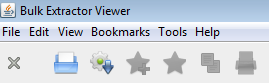
\includegraphics[keepaspectratio=true,scale=0.6]{viewerPics/runBulkSnippet}}
\label{fig:runBulk1}
\end{minipage}

A window will pop up and the first two input boxes allow you to select an Image File and specify an Output Feature Directory to create. Enter both of those and then select the button at the bottom of the window titled "Start bulk\_extractor" to run \bulk.
[See \textbf{\Autoref{RunningViewer}} \textbf{\nameref{RunningViewer}}]

\item Whether \bulk was run from the command line or the \viewer tool, after the run the resulting output files will be contained in the specified output directory. Open that directory and verify files have been created. There should be 15-25 files. Some will be empty and others will be populated with data.

\item Users can join the google email users group for more information and help with any issues encountered. Email \textbf{bulk\_extractor-users+subscribe@googlegroups.com} with a blank message to join.
\end{enumerate}
\newpage

\section*{One Page Quickstart for Windows Users}
This page provides a very brief introduction to downloading, installing and running \bulk. 
\begin{enumerate}
\item If you do not already have one, obtain a disk image on which to run \bulk. Sample images can be downloaded from \url{http://digitalcorpora.org/corpora/disk-images}. Suggestions include \texttt{nps-2009-domexusers} and \\ \texttt{nps-2009-ubnist1.gen3}.
\item Download the latest version of the \bulk Windows installer. It can be obtained from \url{http://digitalcorpora.org/downloads/bulk_extractor}. The file to download is called \texttt{bulk\_extractor-x.y.z-windowsinstaller.exe} where x.y.z is the latest version number.  Run the installer file. This will automatically install \bulk on your machine. The automatic installation includes the complete \bulk system as well as the \viewer tool. [See \textbf{\Autoref{InstallOnWindows}} \textbf{\nameref{InstallOnWindows}}]

\item To run \bulk from the command line, type the following command:
\begin{Verbatim}[commandchars=\\\{\}]
\verbbf{bulk_extractor -o output mydisk.raw}
\end{Verbatim} 

In the above command, \textbf{output} is the directory that will be created to store \bulk results.  It can not already exist. The input \textbf{mydisk.raw} is the disk image to be processed.
[See  \textbf{\Autoref{RunFromCommandLine}} \textbf{\nameref{RunFromCommandLine}}]

\item To run \bulk from the \viewer, run the program \textbf{Bulk Extractor X.Y} from the Start Menu. 

In the \viewer, click on the Gear/down arrow icon as depicted below. 
\noindent
\begin{minipage}{\linewidth}
	\makebox[\linewidth]{%
	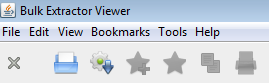
\includegraphics[keepaspectratio=true,scale=0.6]{viewerPics/runBulkSnippet}}
\label{fig:runBulk2}
\end{minipage}

A window will pop up and the first two input boxes allow you to select an Image File and specify an Output Feature Directory to create. Enter both of those and then select the button at the bottom of the window titled "Start bulk\_extractor" to run \bulk.
[See \textbf{\Autoref{RunningViewer}} \textbf{\nameref{RunningViewer}}]

\item Whether \bulk was run from the command line or the \viewer tool, after the run the resulting output files will be contained in the specified output directory. Open that directory and verify files have been created. There should be 15-25 files. Some will be empty and others will be populated with data.

\item Users can join the google email users group for more information and help with any issues encountered. Email \textbf{bulk\_extractor-users+subscribe@googlegroups.com} with a blank message to join.
\end{enumerate}
\newpage


\tableofcontents
\newpage
\pagenumbering{arabic}





\newpage

\section{Introduction}

\subsection{Overview of \bulk}
\bulk is a program that extracts features such as email addresses, credit card numbers, URLs, and other types of information from digital evidence files. It is a useful forensic investigation tool for many tasks such as malware and intrusion investigations, identity investigations and cyber investigations, as well as analyzing imagery and password cracking. The program provides several unusual capabilities including:
\begin{itemize}
\item It finds email addresses, URLs and credit card numbers that other tools miss because it can process compressed data (like ZIP, PDF and GZIP files) and incomplete or partially corrupted data. It can carve JPEGs, office documents and other kinds of files out of fragments of compressed data. It will detect and carve encrypted RAR files.
\item It builds word lists based on all of the words found within the data, even those in compressed files that are in unallocated space. Those word lists can be useful for password cracking.
\item It is multi-threaded; running \bulk on a computer with twice the number of cores typically makes it complete a run in half the time.
\item It creates histograms showing the most common email addresses, URLs, domains, search terms and other kinds of information on the drive.
\end{itemize}

\bulk operates on disk images, files or a directory of files and extracts useful information without parsing the file system or file system structures. The input is split into pages and processed by one or more scanners. The results are stored in feature files that can be easily inspected, parsed, or processed with other automated tools. \bulk also creates histograms of features that it finds. This is useful because features such as email addresses and internet search terms that are more common tend to be important. \\  

In addition to the capabilities described above, \bulk also includes:
\begin{itemize}	
	\item A graphical user interface, \viewer, for browsing features stored in feature files and for launching \bulk scans
	\item A small number of python programs for performing additional analysis on feature files
\end{itemize} 
\bulk 1.5 detects and optimistically decompresses data in ZIP, GZIP, RAR, and Microsoft's Hibernation files. This has proven useful, for example, in recovering email addresses from fragments of compressed files found in unallocated space. \\

\bulk contains a simple but effective mechanism for protecting against decompression bombs. It also has capabilities specifically designed for Windows and malware analysis including decoders for the Windows PE, Linux ELF, VCARD, Base16, Base64 and Windows directory formats.\\

\bulk gets its speed through the use of compiled search expressions and multi-threading. The search expressions are written as pre-compiled regular expressions, essentially allowing \bulk to perform searches on disparate terms in parallel. Threading is accomplished through the use of an analysis thread pool.  After the features have been extracted, \bulk builds a histogram of email addresses, Google search terms, and other extracted features. Stop lists can also be used to remove features not relevant to a case. \\

\bulk is distinguished from other forensic tools by its speed and thoroughness. Because it ignores file system structure, \bulk can process different parts of the disk in parallel. This means that an 8-core machine will process a disk image roughly 8 times faster than a 1-core machine. \bulk is also thorough. It automatically detects, decompresses, and recursively re-processes data that has been compressed with a variety of algorithms. Our testing has shown there is a significant amount of compressed data in the unallocated regions of file systems missed by most forensics tools that are commonly in use today\cite{encodedEvidence}.  Another advantage of ignoring file systems is that \bulk can be used to process any kind of digital media. The program has been used to process hard drives, SSDs, optical media, camera cards, cell phones, network packet dumps, and other kinds of digital information.\\

Between 2005 and 2008, the \bulk team interviewed law enforcement regarding their use of forensic tools. Law enforcement officers wanted a highly automated tool for finding email addresses and credit card numbers (including track 2 information), phone numbers, GPS coordinates and EXIF information from JPEGs, search terms (extracted from URLs), and all words that were present on the disk (for password cracking). The tool needed to run on Windows, Linux and Mac-based systems with no user interaction. It also had to operate on raw disk images, split-raw volumes and E01 files. The tool needed to run at the maximum I/O speed of the physical drive and never crash. Through these interviews, the initial  requirements for the \bulk system were developed. Over the past five years, we have worked to create the tool that those officers desired. \\

\subsubsection{A \bulk Success Story}
One early \bulk success story comes from the City of San Luis Obispo Police Department in the Spring of 2010. The District Attorney filed charges against two individuals for credit card fraud and possession of materials to commit credit card fraud. The defendants were arrested with a computer. Defense attorneys were expected to argue that the defendants were unsophisticated and lacked knowledge to commit the crime. The examiner was given a 250 GB drive the day before the preliminary hearing; typically it would take several days to conduct a proper forensic investigation of that much data.\\

\bulk found actionable evidence in only two and a half hours including the following information:
\begin{itemize}
\item There were over 10,000 credit card numbers on the hard drive (illegal materials).  Over 1000 of the credit card numbers were unique. 
\item The most common email address belonged to the primary defendant (evidence of possession). 
\item The most commonly occurring internet search engine queries concerned credit card fraud and bank identification numbers (evidence of intent). 
\item The most commonly visited websites were in a foreign country whose primary language is spoken by the defendant (evidence of flight risk). 
\end{itemize}
Armed with this data, the defendants were held without bail.\\

As \bulk has been deployed and used in different applications, it has evolved to meet additional requirements. This manual describes use cases for the \bulk system and demonstrates how users can take full advantage of all of its capabilities.

\subsection{Purpose of this Manual}
This User Manual is intended to be useful to new, intermediate and experienced users of \bulk. It provides an in-depth review of the functionality included in \bulk and shows how to access and utilize features through both command line operation and the \viewer. This manual includes working examples with links to the input data (disk images)  used, giving users the opportunity to work through the examples and utilize all aspects of the system. 

\subsection{Conventions Used in this Manual}
This manual uses standard formatting conventions to highlight file names, directory names and example commands. The conventions for those specific types are described in this section. \\

Names of programs including the post-processing tools native to \bulk and third-party tools are shown in \textbf{bold}, as in \textbf{tcpflow}.\\

File names are displayed in a fixed width font. They will appear as \texttt{filename.txt} within the text throughout the manual.\\

Directory names are displayed in italics. They appear as \textit{directoryname/} within the text. The only exception is for directory names that are part of an example command. Directory names referenced in example commands appear in the example command format.\\

Scanner names are denoted with bold, italicized text. They are always specified in lower-case, because that is how they are referred in the options and usage information for \bulk. Names will appear as \textbf{\textit{scannername}}.\\

This manual contains example commands that should be typed in by the user. A command entered at the terminal is shown like this: \begin{Verbatim}[commandchars=\\\{\}]
\verbbf{command}
\end{Verbatim}

The first character on the line is the terminal prompt, and should not be typed. The black square is used as the standard prompt in this manual, although the prompt shown on a users screen will vary according to the system they are using.\\


\section{How \bulk Works}
\bulk finds email addresses, URLS,  and CCNs that other tools miss. This is due in part to the fact that \bulk optimistically decompresses and re-analyzes all data (e.g. zip fragments, gzip browser cache runs). The decompression operates on incomplete and corrupted data until decompression fails. \bulk can also build word lists for password cracking\\

There are three phases of operation in \bulk:  feature extraction, histogram creation, post processing as shown in Figure ~\ref{fig:overviewPic}. The output feature files contain extracted data designed for easy processing by third party programs or use in spreadsheet tools. The \bulk histogram system automatically summarizes features.\\

\begin{figure}
	\center
	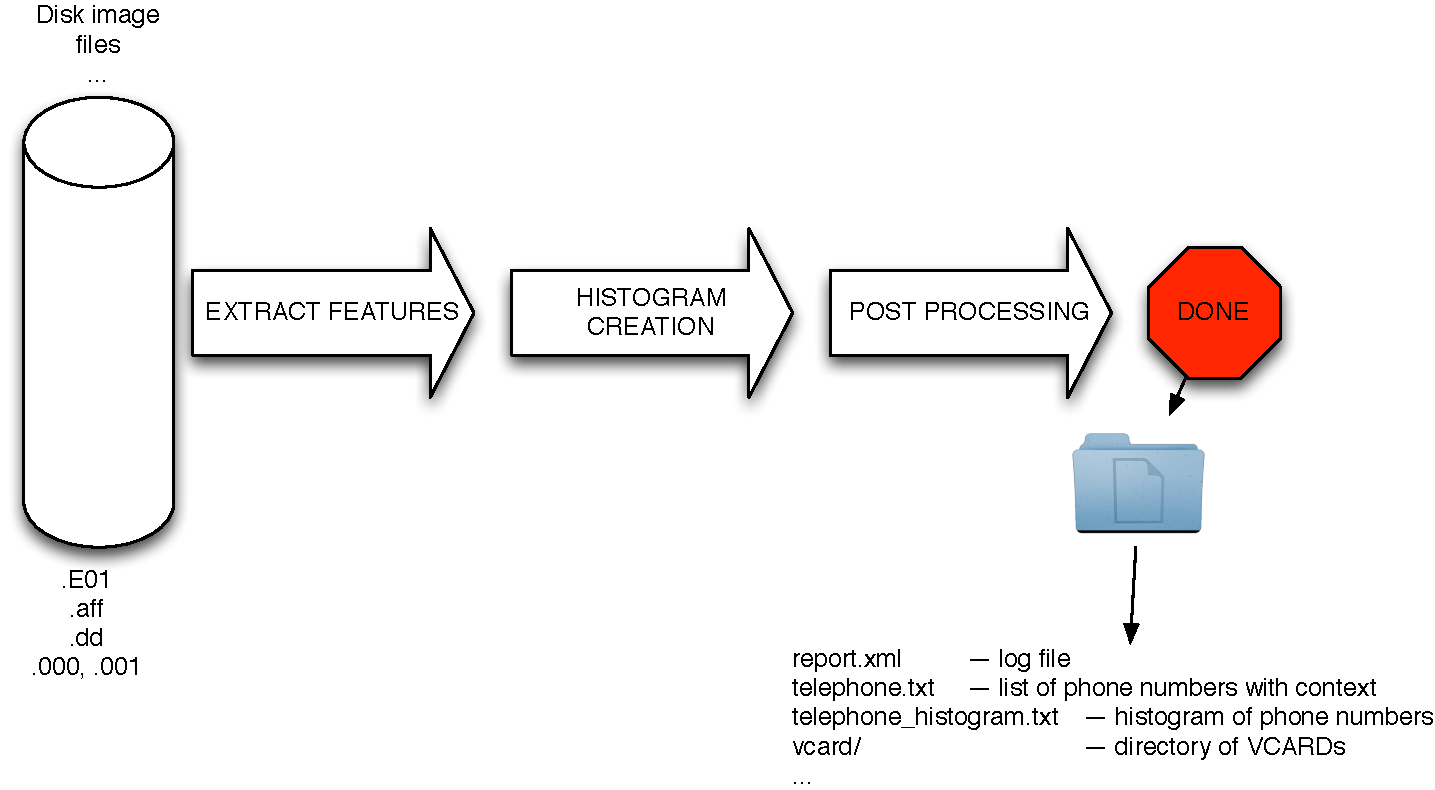
\includegraphics[scale=.60]{archPics/howitworks.pdf}
	\caption{Three Phases of \bulk Operation}
	\label{fig:overviewPic}
\end{figure}

Features files are written using the feature recording system. As features are discovered, they are sent to the feature recorder and recorded in the appropriate file. Multiple scanners might write to the same feature file. For example, the  \textbf{\textit{exif}} scanner searches the file formats used by digital cameras and finds GPS coordinates in images. Those findings are written to the output file \texttt{gps.txt} by the \textbf{\textit{gps}} feature recorder. A separate scanner, the  \textbf{\textit{gps}} scanner, searches Garmin Trackpoint data and also finds GPS coordinates and writes them to \texttt{gps.txt}.  It is worth noting that some scanners also find more than one type of feature and write to several feature files. For example, the  \textbf{\textit{email}} scanner looks for email addresses, domains, URLs and RFC822 headers and writes them to \texttt{email.txt}, \texttt{domain.txt}, \texttt{url.txt}, \texttt{rfc822.txt} and \texttt{ether.txt} respectively.\\

A feature file contains rows of features. Each row is typically comprised of an offset, a feature, and the feature in evidence context although scanners are free to store whatever information they wish. A few lines of an email feature file might look like the following:\\ 
\lstset{style=customfile}
\begin{lstlisting}
OFFSET      FEATURE	        FEATURE IN EVIDENCE CONTEXT
48198832  domexuser2@gmail.com 	__<name>domexuser2@gmail.com/Home
48200361  domexuser2@live.com 	__<name>domexuser2@live.com</name
48413823  siege@preoccupied.net	'Brien  <siege@preoccupied.net>_l
\end{lstlisting}

The types of features displayed in the feature file will vary depending on what type of feature is being stored. However, all feature files use the same format with each row corresponding to one found instance of a feature and three columns describing the related data (offset, feature, and feature in evidence context). \\

Histograms are a powerful tool for understanding certain kinds of evidence. A histogram of emails allows us to rapidly determine the drive's primary user, the user's organization, primary correspondents and other email addresses. The feature recording system automatically makes histograms as data are processed. When the scanner writes to the feature recording system, the relevant histograms are automatically updated. \\ 

A histogram file will, in general, look like the following file excerpt:
\lstset{style=customfile}
\begin{lstlisting}
n=875 mozilla@kewis.ch (utf16=3)
n=651 charlie@m57.biz (utf16=120)
n=605 ajbanck@planet.nl
...
n=288 mattwillis@gmail.com
n=281 garths@oeone.com
n=226 michael.buettner@sun.com (utf16=2)
n=225 bugzilla@babylonsounds.com
n=218 berend.cornelius@sun.com
n=210 ips@mail.ips.es
n=201 mschroeder@mozilla.x-home.org
n=186 pat@m57.biz (utf16=1)
\end{lstlisting}
Each line shows a feature and the number of times that feature was found by \bulk (the histogram indicates how many times the item was found coded as UTF-16). Features are stored in the file in order of occurrence with most frequent features appearing at the top of the file and least frequent displayed at the bottom. \\

\bulk has multiple scanners that extract features. Each scanner runs in an arbitrary order. Scanners can be enabled or disabled which can be useful for debugging and speed optimization. Some scanners are recursive and actually expand the data they are exploring, thereby creating more data that \bulk can analyze. These blocks are called sbufs. The "s" stands for the word safe. All access to data in the sbuf is bounds-checked, so buffer overflow events are very unlikely. The sbuf data structure is one of the reasons that \bulk is so crash resistant. Recursion is used for, among other things, decompressing ZLIB and Windows HIBERFILE, extracting text from PDFs and handling compressed browser cache data. \\

The recursion process requires a new way to describe offsets. To do this, \bulk introduces the concept of the ``forensic path.'' The forensic path is a description of the origination of a piece of data. It might come from, for example, a flat file, a data stream, or a decompression of some type of data. Consider an HTTP stream that contains a GZIP-compressed email as shown in Figure ~\ref{fig:forensicPath}. A series of scanners will first find the ZLIB compressed regions in the HTTP stream that contain the email, decompress them, and then find the features in that email which may include email addresses, names and phone numbers. Using this method, \bulk can find email addresses in compressed data. The forensic path for the email addresses found indicate that it originated in an email, that was GZIP compressed and found in an HTTP stream. The forensic path of the email addresses features found might be represented as follows:
\lstset{style=customfile}
\begin{lstlisting}
11052168704-GZIP-3437  live.com  eMn='domexuser@live.com';var  srf_sDispM
11052168704-GZIP-3475  live.com  pMn='domexuser@live.com';var  srf_sDreCk
11052168704-GZIP-3512  live.com  eCk='domexuser@live.com';var  srf_sFT='<
\end{lstlisting}


\begin{figure}
	\center
	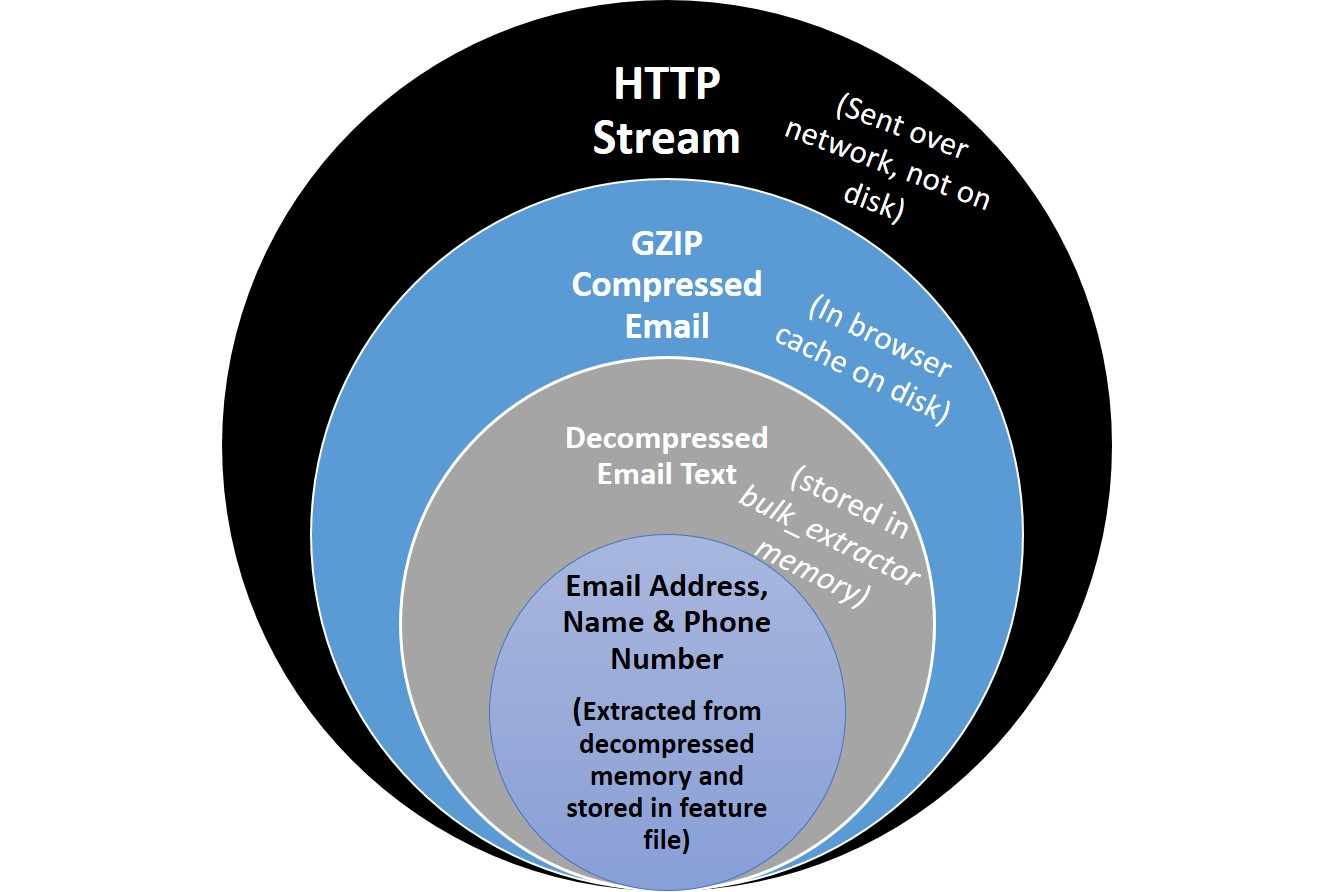
\includegraphics[scale=.60]{otherPics/forensicPath.jpg}
	\caption{Forensic path of features found in email lead back to HTTP Stream}
	\label{fig:forensicPath}
\end{figure}


The full functionality of \bulk is provided both through command line operation and the GUI tool, \viewer.  Both modes of operation work for Linux, Mac and Windows.  The following section describes how to download, install and run \bulk using either the command line or the \viewer.

\section{Running \bulk}
\bulk is a command line tool with an accompanying graphical user interface tool, \viewer. All of the command line functionality of \bulk is also available in the \viewer. Users can access the functionality in whichever way they prefer. In this manual we review the \bulk user options in both formats.\\

\bulk can be run on a Linux, MacOS or Windows system. The fastest way to run \bulk is on a Linux system.  Running on Windows provides the same results, but the run will typically take 40% longer on the same hardware. The software actually runs faster on a Linux virtual machine running on Windows with VMware workstation than on the native Windows OS. 


\subsection{Installation Guide}
Installation instructions vary for Linux/Mac users and Windows users. The following sections explain how to install \bulk.

\subsubsection{Installing on Linux or Mac}
\label{InstallOnLinuxMac}
Before compiling \bulk for your platform, you may need to install other packages on your system which \bulk requires to compile cleanly and with a full set of capabilities.\\

\textbf{Dependencies for Linux Fedora}\\
This command should add the appropriate packages:
\begin{Verbatim}[commandchars=\\\{\}]
\verbbf{sudo yum update}
\verbbf{sudo yum groupinstall development-tools}
\verbbf{sudo yum install flex}
\end{Verbatim}

\textbf{Dependencies for Linux Debian Testing (wheezy) or Ubuntu 13.0}\\
The following command should add the appropriate libraries:
\begin{Verbatim}[commandchars=\\\{\}]
\verbbf{sudo apt-get -y install gcc g++ flex libewf-dev} 
\end{Verbatim}

\textbf{Dependencies for Mac Systems}\\
Mac users must first install Apple's Xcode development system. Other components should be downloaded using the MacPorts system. If you do not have MacPorts, go to the App store and download and install it. It is free. Once it is installed, try:
\begin{Verbatim}[commandchars=\\\{\}]
\verbbf{sudo port install flex autoconf automake libewf-devel}
\end{Verbatim}

Mac users should note that libewf-devel may not be available in ports.  If it is not, download and un-tar the libewf source, cd into the directory and run:
\begin{Verbatim}[commandchars=\\\{\}]
\verbbf{./configure} 
\verbbf{make}
\verbbf{sudo make install}
\end{Verbatim}

\textbf{Download and Install \bulk}\\
Next, download the latest version of \bulk. The software can be downloaded from \url{http://digitalcorpora.org/downloads/bulk_extractor/}. The file to download will be called \texttt{bulk\_extractor-x.y.z.tar.gz} where x.y.z is the latest version. As of publication of this manual, the latest version of \bulk is 1.5.0. \\


After downloading the file, un-tar it. Then, in the newly created \textit{bulk\_extractor-x.y.z} directory, run the following commands to install \bulk in \textit{/usr/local/bin} (by default):

\begin{Verbatim}[commandchars=\\\{\}]
\verbbf{./configure}
\verbbf{make}
\verbbf{sudo make install}
\end{Verbatim}


With these instructions, the following directory will not be installed:
\begin{itemize}
\item{\textit{plugins/} - This is for C/C++ developers only. You can develop your own \bulk plugins which will then be run at run-time with the \bulk executable. Refer to the \textbf{\bulk Programmers Manual for Developing Scanner Plug-ins \cite{programmersmanual}} for more information.}
\end{itemize}
Instructions on running \bulk from the command line can be found in \textbf{\Autoref{RunFromCommandLine}}.\\
	
The \viewer tool is installed as part of the above installation process. Specific instructions on running it can be found in \textbf{\Autoref{RunningViewer}}.

\subsubsection{Installing on Windows}
\label{InstallOnWindows}
Windows users should download the Windows Installer for \bulk.  The file to download is located at \url{http://digitalcorpora.org/downloads/bulk_extractor/executables/} and is called \texttt{bulk\_extractor-x.y.z-windowsinstaller.exe} where x.y.z is the latest version number (1.5.0 as of publication of this manual).   \\

Next, run the \texttt{bulk\_extractor-x.y.z-windowsinstaller.exe} file. This will automatically install \bulk on your machine. Because this file is not used by many Windows users, some anti-virus systems will try to manual delete it on download or block the download as shown in Figure ~\ref{fig:installer_download}.  Be aware that you may have to work around your anti-virus system. Additionally, some Windows versions will try to prevent you from running it. Figure ~\ref{fig:windowsWarning} shows the message Windows 8 displays when trying to run the installer. To run anyway, click on ``More info'' and then select ``Run Anyway.''\\
\begin{figure}
	\center
	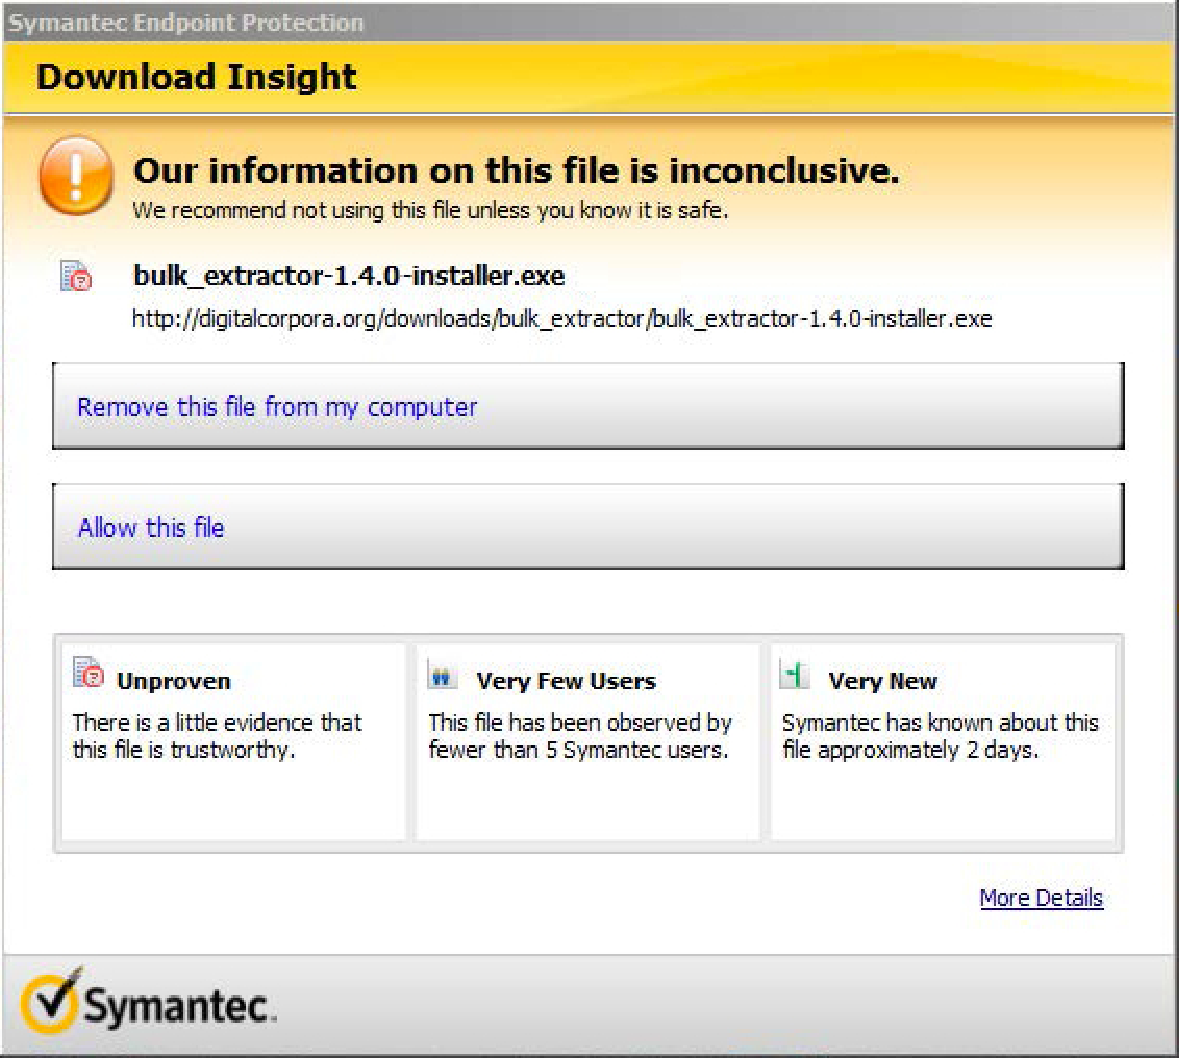
\includegraphics[scale=.60]{installPics/installer_download.pdf}
	\caption{Anti-virus software, such as Symantec, often tries to block download of the installer file}
	\label{fig:installer_download}
\end{figure}

\begin{figure}
	\center
	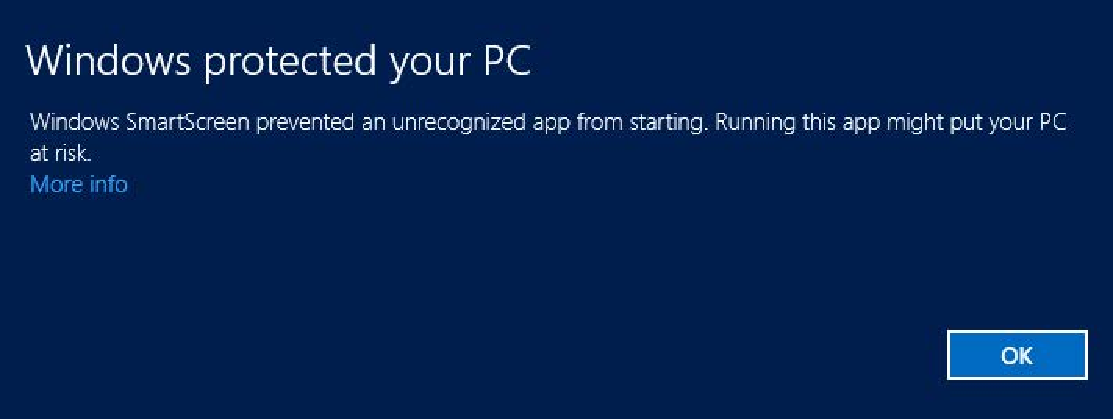
\includegraphics[scale=.50]{installPics/windowsWarning2.pdf}
	\caption{Windows 8 warning when trying to run the installer}
	\label{fig:windowsWarning}
\end{figure}

When the installer file is executed, the installation will begin and show a dialog like the one shown in Figure ~\ref{fig:installer1}.  Users should select the default configuration, which will be the 64-bit configuration for 64-bit Windows systems, or the 32-bit configuration for 32-bit Windows systems.  Click on ``Install'' and the installer will install \bulk on your system and then notify you when it is complete.\\
\begin{figure}
	\center
	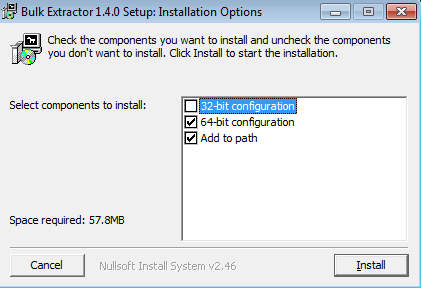
\includegraphics[scale=.70]{installPics/installer1.png}
	\caption{Dialog appears when the user executes the Windows Installer}
	\label{fig:installer1}
\end{figure}


The automatic installation includes the \viewer tool as well as the complete \bulk system that can be run from the command line. Java 6 or above must  be installed on the machine for the \viewer to run. Instructions on running \bulk from the command line can be found in  \textbf{\Autoref{RunFromCommandLine}}. Instructions on running it from the \viewer are located in \textbf{\Autoref{RunningViewer}}. \\

\subsection {Run \bulk from the Command Line}
\label{RunFromCommandLine}
The two main parameters required to run \bulk are an output directory and a disk image. The output directory must be a directory that does not already exist. The disk image can be either a file such as a disk image or a directory of individual files. \bulk cannot process a directory of disk images.\\

In the following instructions, \textit{output} is the name of the directory that will be created to store the \bulk output. The file \texttt{mydisk.raw} is the name of the disk image that will be extracted by \bulk. \\

To run \bulk from the command line on any machine, type the following command:
\begin{Verbatim}[commandchars=\\\{\}]
\verbbf{bulk_extractor -o output mydisk.raw}
\end{Verbatim}

The above command on any of the supported operating systems assumes that the disk image \textit{mydisk.raw} is located in the directory where the command is being executed. However, you can point \bulk to a disk image found elsewhere on your machine by explicitly entering the path to that image.\\

The following text shows the output that is produced when \bulk is run on the file \texttt{nps-2010-emails.E01}. The information printed indicates the version number, input file, output directory and disk size. The screen is updated as \bulk runs  with status information. \bulk then prints performance information and the number of features found when the run is complete.

\begingroup
\footnotesize
\texttt{C:\textbackslash \textgreater \textbf{bulk\_extractor -o bulk\_extractor\textbackslash Output\textbackslash nps-2010-emails bulk\_extractor\textbackslash In\\putData\textbackslash nps-2010-emails.E01}}
\endgroup
\begingroup
\footnotesize
\begin{Verbatim}[fontfamily=courier]
bulk_extractor version: 1.5.0
Input file: bulk_extractor\InputData\nps-2010-emails.E01
Output directory: bulk_extractor\Output\nps-2010-emails
Disk Size: 10485760
Threads: 4
All data are read; waiting for threads to finish...
Time elapsed waiting for 1 thread to finish:
     (timeout in 60 min .)
Time elapsed waiting for 1 thread to finish:
    6 sec (timeout in 59 min 54 sec.)
Thread 0: Processing 0

All Threads Finished!
Producer time spent waiting: 0 sec.
Average consumer time spent waiting: 8.32332 sec.
Phase 2. Shutting down scanners
Phase 3. Creating Histograms
   ccn histogram...   ccn_track2 histogram...   domain histogram...
   email histogram...   ether histogram...   find histogram...
   ip histogram...   lightgrep histogram...   tcp histogram...
   telephone histogram...   url histogram...   url microsoft-live...
   url services...   url facebook-address...   url facebook-id...
   url searches...Elapsed time: 11.1603 sec.
Overall performance: 0.939557 MBytes/sec
Total email features found: 67
\end{Verbatim}
\endgroup

Note that \bulk has automatically selected to use 4 threads; this is because the program was run on a computer with 4 cores. In general, \bulk automatically determines the correct number of cores to use. It is not necessary to set the number of threads to use.\\

After running \bulk, examine the output directory specified by name in the run command. There should now be a number of generated output files in that directory. There are several categories of output created for each \bulk run. First, there are feature files grouped by category, which contain the features found and include the path, feature and context. Second, there are histogram files that allow users to quickly see the features grouped by the frequency in which they occur. Certain kinds of files, such as JPEGs and KML files, may be carved into directories. Finally, \bulk creates a file \texttt{report.xml}, in DFXML format, that captures the provenance of the run. After \bulk has been run, all of these files will be found in the output directory specified by the user.\\

The text below shows the results of running the command \textbf{ls -s} within the output directory from the \bulk run on the disk image \texttt{nps-2010-emails.E01}. The numbers next to the file names indicate the file size and show that several of the files, including \texttt{email.txt} and \texttt{domain.txt}, were populated with features during the run.

\begingroup
\footnotesize
\texttt{C:\textbackslash bulk\_extractor\textbackslash Output\textbackslash nps-2010-emails\textgreater \textbf{ls -s}}
\endgroup
\begingroup
\footnotesize
\begin{Verbatim}[fontfamily=courier]
total 303
 0 aes_keys.txt               0 kml.txt
 0 alerts.txt                 0 lightgrep.txt
 0 ccn.txt                    0 lightgrep_histogram.txt
 0 ccn_histogram.txt          0 rar.txt
 0 ccn_track2.txt             8 report.xml
 0 ccn_track2_histogram.txt   0 rfc822.txt
64 domain.txt                 0 tcp.txt
 1 domain_histogram.txt       0 tcp_histogram.txt
 0 elf.txt                    0 telephone.txt
16 email.txt                  0 telephone_histogram.txt
 4 email_histogram.txt       96 url.txt
 0 ether.txt                  0 url_facebook-address.txt
 0 ether_histogram.txt        0 url_facebook-id.txt
 1 exif.txt                   4 url_histogram.txt
 0 find.txt                   0 url_microsoft-live.txt
 0 find_histogram.txt         0 url_searches.txt
 0 gps.txt                    1 url_services.txt
 0 hex.txt                    0 vcard.txt
 0 ip.txt                    12 windirs.txt
 0 ip_histogram.txt           0 winpe.txt
 0 jpeg                       0 winprefetch.txt
 8 jpeg_carved.txt            88 zip.txt
 0 json.txt
\end{Verbatim}
\endgroup


There are numerous feature files produced by \bulk for each run. A feature file is a tab-delimited file that show a feature on each row. Each row includes a path, a feature and the context. The files are in UTF-8 format.\\

Any of the feature files created by \bulk may have an accompanying \texttt{*\_stopped.txt} file found in the output directory. This file will show all stopped entries of that type that have been found so that users can examine those files to make sure nothing critical has been hidden. A stopped features is a feature that appears in a stop list. The stop list is a list of features that are not of concern for a particular investigation. For example, users may input a stop list file to \bulk that contains numerous email addresses that should be ignored and not marked as a found feature. Rather than throwing away those results when they are found, \bulk will create a file, named \texttt{email\_stopped.txt} that shows all email addresses from the stop list that were found during the run. The stopped email addresses will not show up in the \texttt{email.txt} file. More information on creating and using stop lists can be found in \textbf{\Autoref{StoppedLists}}.\\

While the above commands are all that is required for basic operation, there are numerous usage options that allow the user to affect input and output, tuning, path processing mode, debugging, and control of scanners. All of those options are described when \bulk is run with the -h (help) option. It is important to note that the overwhelming tendency of users is to use many of these options; \textbf{however}, that is not generally recommended. Most of the time, the best way to run \bulk is with no options specified other than -o to specify the output directory. For best performance and results users should avoid adding them in general. Only advanced sers in specific cases should use these options.\\

Running \bulk with only the -h option specified produces the output shown in \textbf{\Autoref{HelpOutput}}.  To run any optional usage options, they should be inserted before the input and output options are specified. Specifically, the order should look like the following:

\begin{Verbatim}[commandchars=\\\{\}]
\verbbf{bulk_extractor [Usage Options] -o output mydisk.raw}
\end{Verbatim}

The specific order in which multiple usage options are specified matters. Some of the options are discussed within the following sections for specific use cases, other options are for programmer or experimental use. In general, avoid using the options unless indicated for a specific purpose.\\

\subsection{Run \bulk from \viewer}
\label{RunningViewer}

On a Linux or Mac system, go to the directory where the \viewer is installed or specify the full path name to the jar file. It will be in the location where the \bulk code was installed and in the sub-directory labeled \textit{java\_gui}. From that directory, run the following command to start the \viewer:
\begin{Verbatim}[commandchars=\\\{\}]
\verbbf{./BEViewer}
\end{Verbatim}

\subsection {Run \bulk from Bulk Extractor Viewer}

Windows users should go to the Start menu and choose Programs->Bulk\_Extractor x.y.z->BE Viewer with Bulk\_extractor x.y.z (64-bit). If the 64-bit version can not be run on your machine, you can choose the 32-bit version. The Troubleshooting section describes some limits users of the 32-bit version might encounter.\\

When the \viewer starts up, it will look like Figure ~\ref{fig:startup}. The look and feel may vary slightly according to the specific operating system but all options should appear similar. To run \bulk from the viewer, click on the icon that looks like a gear with a down arrow. It is next to the Print icon below the Tools menu. Clicking on this icon will bring up the ``Run bulk\_extractor'' Window as shown in Figure ~\ref{fig:runBulk3}.\\
\begin{figure}
	\center
	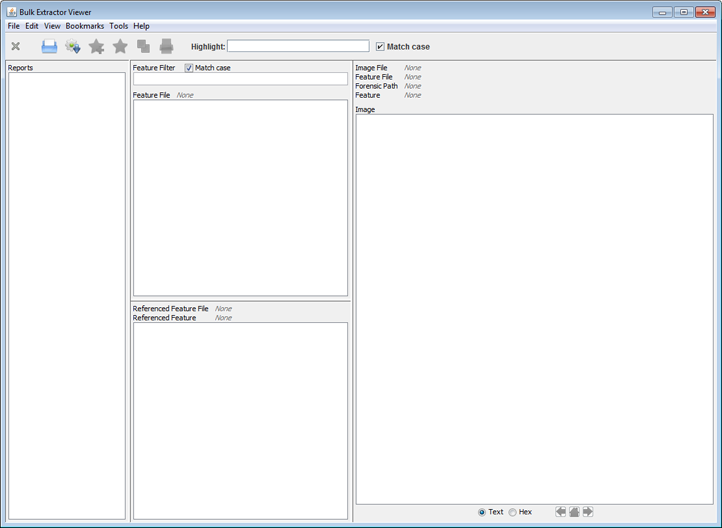
\includegraphics[scale=.8]{viewerPics/startup.png}
	\caption{What \viewer looks like when it is started}
	\label{fig:startup}
\end{figure}


\begin{figure}
	\center
	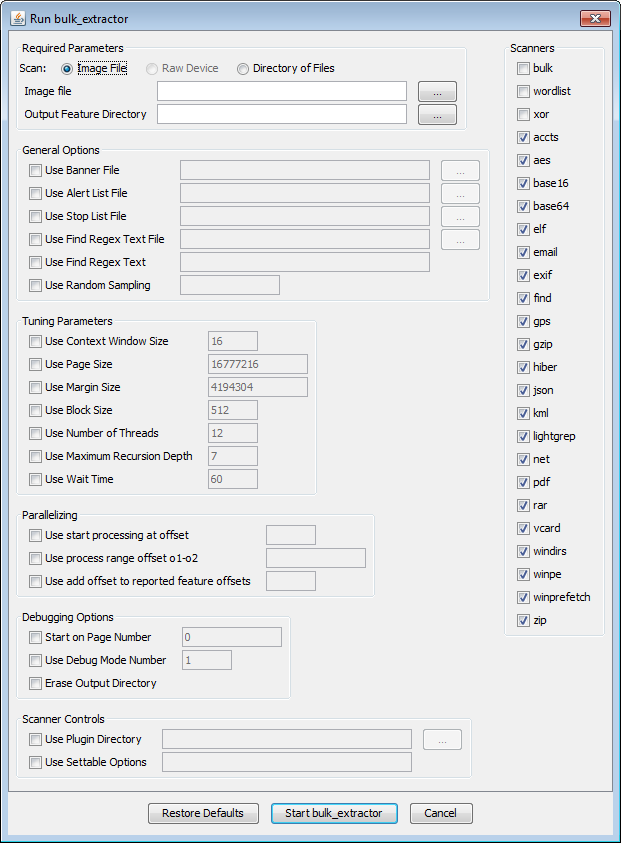
\includegraphics{viewerPics/runBulk.png}
	%\captionsetup{font=LARGE}
	\caption{Clicking on the gear icon brings up this ``Run bulk\_extractor'' Window}
	\label{fig:runBulk3}
\end{figure}

Next, in the ``Run bulk\_extractor'' window select the Image File and Output Feature Directory to run \bulk. Figure ~\ref{fig:selectOutputDirectory} shows an example where the user has selected the file \texttt{nps-2010-emails.E01} as input and is going to create a directory called \textit{nps-2010-charlie-output} in the parent directory \textit{C:\textbackslash bulk\_extractor\textbackslash Output}. Note that figures may vary slightly in future versions of \bulk but the major functionality will remain the same.\\
\begin{figure}
    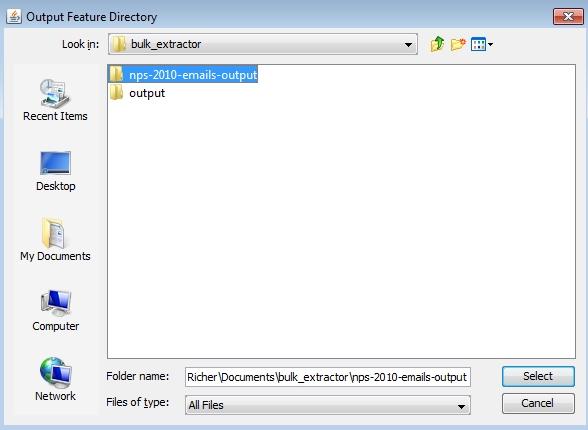
\includegraphics[scale=.8]{viewerPics/selectOutputDirectory.png}
	\caption{After selecting an Image File for input, the user must select an output directory to create}
	\label{fig:selectOutputDirectory}
\end{figure}
 
After selecting the input and output directories, click on the button at the bottom of the ``Run bulk\_extractor'' window labeled ``Start bulk\_extractor.'' This will bring up the window shown in Figure ~\ref{fig:runCompleteStatus} that updates as \bulk is running, providing status information during the run and after the run is complete. \\
\begin{figure}
	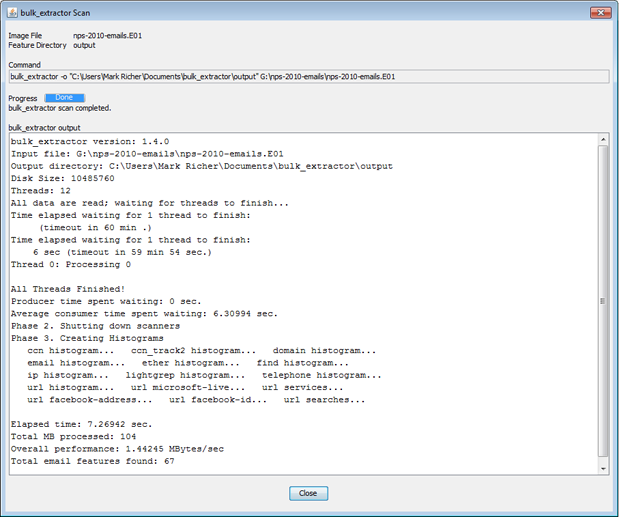
\includegraphics{viewerPics/runCompleteStatus.png}
	\caption{Status window that shows what happens as \bulk runs and indicates when \bulk is complete}
	\label{fig:runCompleteStatus}
\end{figure}

When the run is complete, a dialog will pop-up indicating the results are ready to be viewed. Figure ~\ref{fig:reportIsReady} shows this dialog. Click the ``Ok'' button which will return you to the main \viewer window to view the results of the run. The ``Reports'' window on the left will now show the newly created report. In this example, the report is called ``nps-2010-emails-output.'' Clicking once on this report name will expand the report and show all of the files that have been created as shown in Figure ~\ref{fig:listOfOutput}. \\
\begingroup
\center
\begin{figure}
	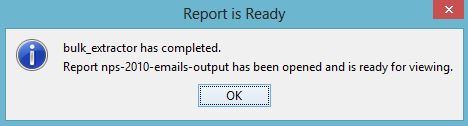
\includegraphics{viewerPics/reportIsReady.png}
	\caption{Dialog indicating the run of \bulk is complete and results are ready to be viewed}
	\label{fig:reportIsReady}
\end{figure}
\endgroup
\begin{figure}
	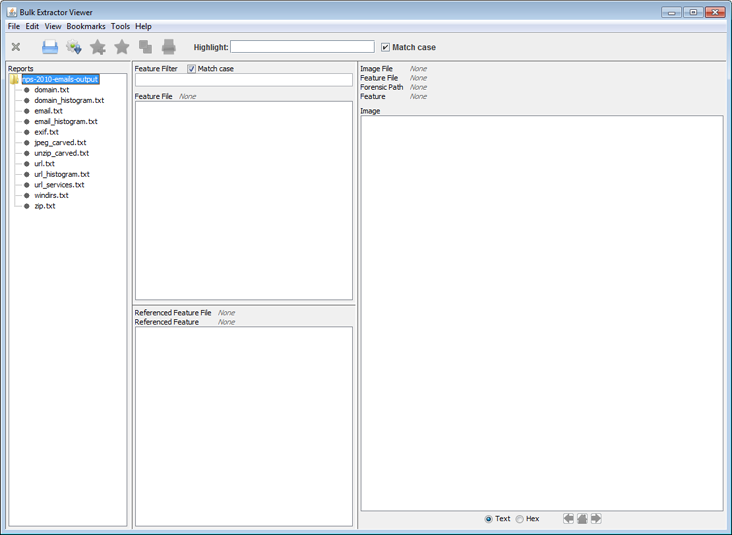
\includegraphics[scale=.8]{viewerPics/listOfOutput.png}
	\caption{Reports window shows the newly created report and all of the files created in that report}
	\label{fig:listOfOutput}
\end{figure}
Clicking on one of the files will bring that file up in the ``Feature File'' window in the middle of the screen. In the example, the user clicked on \texttt{email.txt} to view the email feature file. Clicking on one of the features, in this case \textbf{rtf\_text@textedit.com}, shows the feature in context within the feature file on the right hand side of the window as shown in Figure ~\ref{fig:emailFeatureFile}.\\

\begin{figure}
	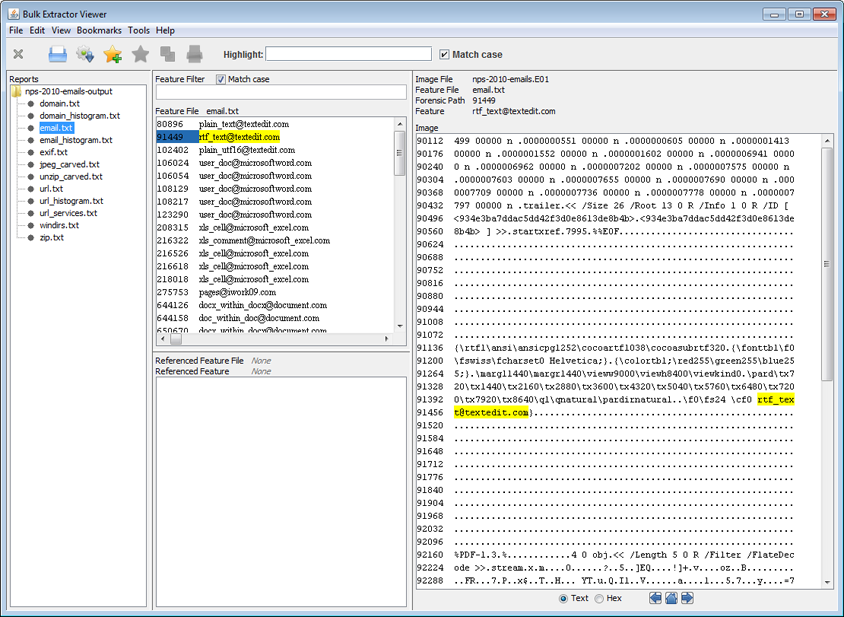
\includegraphics[scale=.7]{viewerPics/emailFeatureFile.png}
	\caption{While viewing the feature file, the user can select a feature to view with it's full context in the feature file as shown in the right hand side of the window}
	\label{fig:emailFeatureFile}
\end{figure}

The user can also view histogram files in the \viewer. Clicking on the file, \texttt{email\_histogram.txt} in the Reports window on the left hand side will bring up the contents of the histogram file in the middle window. It will also display the referenced feature file in the window below the histogram file. In this case, the referenced feature file is \texttt{email.txt}. Clicking on a feature in the histogram, in this example \textbf{rtf\_text@textedit.com}, will display the feature in context as found within the feature file on the right hand side of the screen as shown in Figure ~\ref{fig:emailHistogramView}.\\

\begin{figure}
	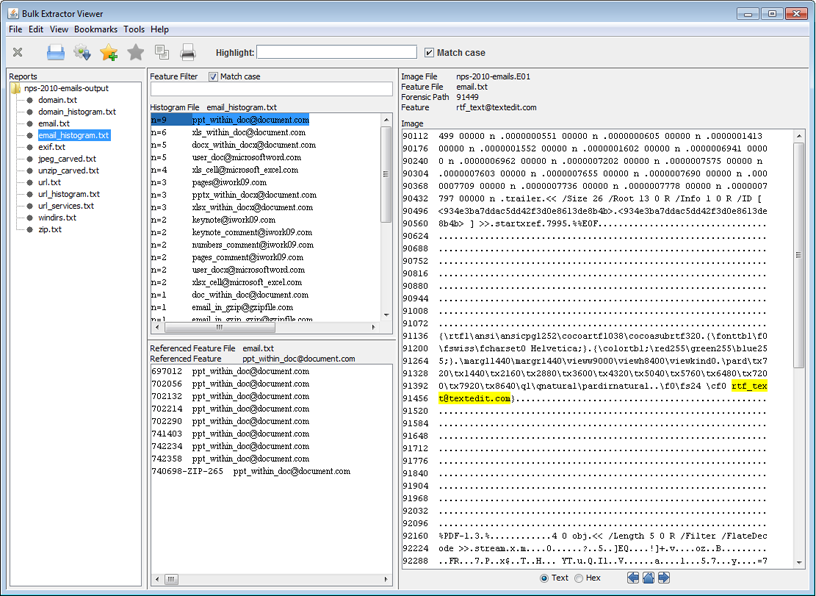
\includegraphics[scale=.70]{viewerPics/emailHistogramView.png}
	\caption{User can view histograms of features, referenced feature files and specific features in context}
	\label{fig:emailHistogramView}
\end{figure}


\section{Processing Data}
\subsection{Types of Input Data}

The \bulk system can handle multiple image formats including E01, raw, split raw and individual disk files as well as raw devices or files.  It can also operate on memory and packet captures, although packet captures will be more completely extracted if you pre-process them with \textbf{tcpflow}.\\

The scanners all serve different functions and look for different types of information. Often, a feature will be stored in a format not easily accessible and will require multiple scanners to extract the feature data. For example, some PDF files contain text data but the PDF format is not directly searchable by the scanner that finds email addresses or the scanner that looks for keywords. \bulk resolves this by having the two scanners work together. The \textbf{\textit{pdf}} scanner will first extract all of the text from the PDF and then the other scanners will look at the extracted text for features. This is important to remember when turning scanners off and on, as scanners work together to retrieve the features from the disk image. The types of information examined, extracted or carved by the existing \bulk scanners are as described in Table ~\ref{tab:inputdata}, along with the scanners that process them and the specific sections where they are referenced in this manual.

\begin{longtable}{|p{2 cm}|p{6cm}|p{3 cm}|}
\caption{Input Data Processed by the Scanners}\\
\hline
\textbf{Scanner Name} & \textbf{Data Type} & \textbf{Section Discussed in Manual} \\
\endfirsthead
\hline
\textbf{Scanner Name} & \textbf{Data Type} & \textbf{Section Discussed in Manual} \\
\endhead
\hline
\endfoot
\hline
\endlastfoot

\label{tab:inputdata}
\hline\textbf{\textit{accts}} & Numeric accounts, such as phone numbers and CCNs\\
\hline\textbf{\textit{aes}} & In-memory AES keys from their key schedules & \Autoref{cyber}\\
\hline\textbf{\textit{base16}} & Base 16 (hex) encoded data (includes MD5 codes embedded in the data) & \Autoref{cyber}\\
\hline\textbf{\textit{base64}} & Base 64 code & \Autoref{compressedProcessing} and \Autoref{cyber} \\
\hline\textbf{\textit{elf}} & Executable and Linkable Format (ELF) & \Autoref{malware} \\
\hline\textbf{\textit{exif}} & EXIF structures from JPEGS (and carving of JPEG files) & \Autoref{imagery} \\
\hline\textbf{\textit{facebook}} & Facebook HTML & \\
\hline\textbf{\textit{gps}} & XML from Garmin GPS devices (processed) & \Autoref{identity}\\
\hline\textbf{\textit{gzip}} & GZIP files and ZLIB-compressed GZIP streams & \Autoref{compressedProcessing} and \Autoref{cyber} \\
\hline\textbf{\textit{hashdb}} & NPS Hash Database support\\
\hline\textbf{\textit{hiber}} & Windows Hibernation File Fragments (decompressed and processed, not carved) & \Autoref{compressedProcessing}  \\
\hline\textbf{\textit{httplogs}} & HTTP log files\\
\hline\textbf{\textit{jpeg}} & JPEG carving. Default is only encoded JPEGs are carved. JPEGs without EXIFs are also carved & \Autoref{carving} and \Autoref{imagery}\\
\hline\textbf{\textit{json}} & JavaScript Object Notation files and objects downloaded from web servers, as well as JSON-like objects found in source code & \Autoref{malware}\\
\hline\textbf{\textit{kml}} & KML files (carved) & \Autoref{identity}\\
\hline\textbf{\textit{outlook}} & Outlook Compressable Encryption\\
\hline\textbf{\textit{pdf}} & Text from PDF files (extracted for processing not carved) & \Autoref{compressedProcessing} \\
\hline\textbf{\textit{rar}} &  RAR components in unencrypted archives are decrypted and processed. Encrypted RAR file are carved. & \Autoref{carving} \\
\hline\textbf{\textit{sqlite }} & SQLite3 database file detection and carving\\
\hline\textbf{\textit{vcard}} & vCard files (carved) & \Autoref{identity}\\
\hline\textbf{\textit{windirs}} & Windows FAT32 and NTFS directory entries& \Autoref{cyber}\\
\hline\textbf{\textit{winlnk}} & Windows LNK file carving and decoding\\
\hline\textbf{\textit{winpe}} & Windows Preinstallation Environment (PE) Executables (.exe and .dll files notated with MD5 hash of first 4k) & \Autoref{malware}\\
\hline\textbf{\textit{winprefetch}} & Windows Prefetch files, file fragments (processed) & \Autoref{malware} \\
\hline\textbf{\textit{zip}} & ZIP files and zlib streams (processed, and optionally carved) & \Autoref{carving} and \Autoref{compressedProcessing}\\
\hline
\end{longtable}

\subsection{Scanners}
\label{Scanners}
There are multiple scanners deployed with the \bulk system. For a detailed list of the scanners installed with your version of \bulk, run the following command:
\begin{Verbatim}[commandchars=\\\{\}]
\verbbf{bulk_extractor -H}
\end{Verbatim}

This command will show all of the scanners installed with additional information included about each scanner. Specifically, there is a description for each scanner, a list of the features it finds and any relevant flags. A sample of the output is below: 
\begingroup
\footnotesize
\begin{Verbatim}[fontfamily=courier]
Scanner Name: accts
flags:  NONE
Scanner Interface version: 3
Author: Simson L. Garfinkel
Description: scans for CCNs, track 2, and phone #s
Scanner Version: 1.0
Feature Names: alerts ccn ccn_track2 telephone

Scanner Name: base16
flags:  SCANNER_RECURSE
Scanner Interface version: 3
Author: Simson L. Garfinkel
Description: Base16 (hex) scanner
Scanner Version: 1.0
Feature Names: hex

...

Scanner Name: wordlist
flags:  SCANNER_DISABLED
Scanner Interface version: 3
Author:
Description:
Scanner Version:
Feature Names: wordlist
\end{Verbatim}
\endgroup

This output shows that the  \textbf{\textit{accts}} scanner looks for credit card numbers, credit card track 2 information and phone numbers and finds the feature names alerts, ccn, ccn\_track2 and telephone. This means it writes to the feature files \texttt{alerts.txt}, \texttt{ccn.txt}, \texttt{ccn\_track2.txt}, and \texttt{telephone.txt}.\\

The output also shows that the  \textbf{\textit{base16}} scanner is a recursive scanner (indicated by the flag SCANNER\_RECURSE) meaning it expands data or finds new data for other scanners to process. It also writes to the file \texttt{hex.txt}.\\

Finally, the output shows that the  \textbf{\textit{wordlist}} scanner is disabled by default (indicated by the flag SCANNER\_DISABLED). This means that if the user would like to use the  \textbf{\textit{wordlist}} scanner, it will have to be specifically enabled. The wordlist scanner is useful for password cracking and is discussed in \textbf{\Autoref{PasswordCracking}}. \\

In general, most users will not need to enable or disable scanners. The default settings installed with the \bulk system work best for the majority of users. However, individual scanners can be enabled or disabled for different purposes. To enable the  \textbf{\textit{wordlist}} scanner, which is disabled by default, use the following command:
\begin{Verbatim}[commandchars=\\\{\}]
\verbbf{bulk_extractor -e wordlist -o output diskimage.raw}
\end{Verbatim} 

Additionally, users can disable a scanner that is enabled by default. Most of the scanners are enabled by default. To disable the  \textbf{\textit{accts}} scanner, which is very CPU intensive, run the following command:
\begin{Verbatim}[commandchars=\\\{\}]
\verbbf{bulk_extractor -x accts -o output diskimage.raw} 
\end{Verbatim}

The command -E disables all scanners, then enables the one that follows the option. For example, to disable all scanners except the \textbf{\textit{aes}} scanner, use the following command:
\begin{Verbatim}[commandchars=\\\{\}]
\verbbf{bulk_extractor -E aes -o output diskimage.raw}
\end{Verbatim} 

The options -E, -e and -x are all processed in order. So, the following command will also disable all scanners and then enable the \textbf{\textit{aes}} scanner: 
\begin{Verbatim}[commandchars=\\\{\}]
\verbbf{bulk_extractor -x all -e aes -o output diskimage.raw}
\end{Verbatim} 

Some of the scanners installed with \bulk have parameters that can be set and utilized by advanced users for different purposes. Those parameters are also described in the -H output described above (as well as the -h output) and include the following:
\begingroup
\footnotesize
{
\fontfamily{courier}\selectfont
\verbatiminput{SettableOptions.txt}
}
\endgroup

To use any of these options, the user should specify the -S with the name=value pair when running \bulk as in the following example:
\begin{Verbatim}[commandchars=\\\{\}]
\verbbf{bulk_extractor -S name=value -o output diskimage.raw}
\end{Verbatim} 
As with the other scanner and \bulk usage options, most users will not have to use any of these options. 

\subsection{Carving}
\label{carving}

File carving is a special kind of carving in which files are recovered. File carving is useful for both data recovery and forensic investigations because it can recover files when sectors containing file system metadata are either overwritten or damaged \cite{digitalmediatriage}. Currently, \bulk provides carving of contiguous JPEG, ZIP and RAR files. To carve fragmented files we recommend \textbf{PhotoRec} (free) or \textbf{Adroit Photo Recovery}( commercial). Additionally, \textbf{Forensics Toolkit} and \textbf{EnCase Forensic} provide some carving capability on fragmented files.\\

Carved results are stored in two different places. First, a file listing all the files that are carved are written to a corresponding .txt file: JPEG files to \texttt{jpeg\_carved.txt}, ZIP files to \texttt{unzip.txt} and RAR files to \texttt{unrar.txt}. Second, the carved JPEG, ZIP and RAR files are placed in binned directories that are named \textit{/jpeg}, \textit{/unzip} and \textit{/unrar} respectively. For example, all carved JPEGs will go in the directory \textit{/jpeg}. The output files are further binned with 1000 files in each directory. The directory names are 3 decimal digits. If there are more than 999,000 carved files of one type, then the next set of directories are named with 4 digits. File names for JPEGs are the forensicpath.jpg. File names for the ZIP carver are the forensicpath\_filename. If the ZIP file name has slashes in it (denoting directories), they are turned into '\_' (underbars). For example, the file \texttt{mydocs/output/specialfile} will be named \texttt{mydocs\_output\_specialfile}. \\

\begin{table}[!ht]
\centering
\caption{There are three carving modes in \bulk that are specified separately for each file type, JPEG, ZIP and RAR.}
\label{tab:encodings}
\begin{tabular}{|m{2 cm}|m{7 cm}|}
\hline \hline
\textbf{Mode} & \textbf{Mode Description} \\
\hline
0 & Do not carve files of the specified type.\\
\hline
1 & Only carve encoded files of the specified type \\
\hline
2 & Carve everything of the specified type.\\
\hline
\end{tabular}
\end{table}

As the above table describes, there are three carving modes in \bulk that can be specified separately for each file type, JPEG, ZIP or RAR. The first mode, mode 0, explicitly tells \bulk not to carve files of that type. The second mode, mode 1, is on by default and tells \bulk to carve only encoded files of that type. If the user is running the ZIP carver in mode 1 and there is a simple ZIP file, it will not get carved. However, if there is an encoded attachment of that file (like Base64) it will get carved. The final mode, mode 2, will carve everything of that type. There is no way to specify which types of files (particular extensions) will get carved and which will not in mode 2. For example, \bulk will carve both JPEGs and doc files. It carves whatever is encountered.\\

To specify the carving modes for \bulk, command line arguments can be specified. To modify the JPEG carving modes, type the following where carve mode 1=default value that does not need to be specified (carve encoded), 0=no carving or 2=carve everything:
\begin{Verbatim}[commandchars=\\\{\}]
\verbbf{bulk_extractor -S jpeg_carve_mode=1 -o output diskimage.raw}
\end{Verbatim} 
To modify the ZIP carving modes, type the following  where carve mode 1=default value that does not need to be specified (carve encoded), 0=no carving or 2=carve everything:
\begin{Verbatim}[commandchars=\\\{\}]
\verbbf{bulk_extractor -S zip_carve_mode=1 -o output diskimage.raw}
\end{Verbatim} 
To modify the RAR carving modes, type the following  where carve mode 1=default value that does not need to be specified (carve encoded), 0=no carving or 2=carve everything:
\begin{Verbatim}[commandchars=\\\{\}]
\verbbf{bulk_extractor -S rar_carve_mode=1 -o output diskimage.raw}
\end{Verbatim} 
Any combination of the carving mode options can be specified for a given run. The carvers can run in any combination of modes. For example, the JPEG carver can be run in mode 2 while the RAR carving is turned off in mode 1 and the ZIP carver carves only encoded files in mode 1.\\

Because \bulk can carve files and preserve original file extensions, there is a real possibility that \bulk might be carving out malware. There is no protection in \bulk against putting malware in a file on your hard drive. Users running \bulk to look for malware should turn off all anti-virus software because the anti-virus program will think its creating malware and stop it. Then the user should carefully scan the results looking for malware before re-enabling the anti-virus. \\


\subsection{Suppressing False Positives}
\label{StoppedLists}
Modern operating systems are filled with email addresses. They come from Windows binaries, SSL certificates and sample documents. Most of these email addresses, particularly those that occur the most frequently, such as someone@example.com, are not relevant to the case. It is important to be able to suppress those email addresses not relevant to the case. To address this problem, \bulk provides two approaches. \\

First, \bulk allows users to build a stop list or use an existing one available for download. These stop lists are used to recognize and dismiss the email addresses that are native to the Operating System. This approach works well for email addresses that are clearly invalid, such as someone@example.com. For most email addresses, however, you will want to stop them in some circumstances but not others. For example, there are over 20,000 Linux developers, you want to stop their email addresses in program binaries, not in email messages.\\

To address this problem, \bulk uses context-sensitive stop lists. Instead of a stop list of features, this approach uses the feature+context. The following example is an excerpt from a context-sensitive stop list file.

\lstset{style=customfile}
\begin{lstlisting}
ubuntu-users@lists.ubuntu.com   Maint\x0A935261357\x09ubuntu-users@lists.ubuntu.com\x0
ubuntu-motu@lists.ubuntu.com    untu_\x0A923867047\x09ubuntu-motu@lists.ubuntu.com\x09
pschiffe@redhat.com     Peter Schiffer <pschiffe@redhat.com> - 0.8-1.1N\x94/\xC0-
phpdevel@echospace.com  :  Vlad Krupin <phpdevel@echospace.com>\x0AMAINTENANCE:
anholt@freebsd.org      34-GZIP-1021192\x09anholt@freebsd.org\x09r: EricAnholt
ubuntu-motu@lists.ubuntu.com     http\x0A938966489\x09ubuntu-motu@lists.ubuntu.com\x09
\end{lstlisting}

The context for the feature is the 8 characters on either side of the feature. Each ``stop list'' entry is the feature+context. This ignores Linux developer email addresses in Linux binaries. The email address will be ignored if found in that context but reported if it appears in a different context. \\

There is a context-sensitive stop list for Microsoft Windows XP, 2000, 2003, Vista and several Linux systems. The total stop list is 70 MB and includes 628,792 features in a 9 MB zip file. The context-sensitive stop list prunes many of the OS-supplied features. By applying it to the domexusers HD image (the image can be downloaded at \url{http://http://digitalcorpora.org/corp/nps/drives/nps-2009-domexusers/}, the number of emails found went from 9,143 down to 4,459. This significantly reduces the amount of work to be done by the investigator. Figure ~\ref{fig:withandwithoutstoplist} shows how the histogram of email addresses differs when \bulk is run with and without the context-sensitive stop list. The context-sensitive stop list built for the various operating systems described above can be downloaded from \url{http://digitalcorpora.org/downloads/bulk_extractor}. The file will have the words ``stoplist'' in it somewhere. The current version as of publication of this manual is called \texttt{bulk\_extractor-3-stoplist.zip}.

\begin{figure}
	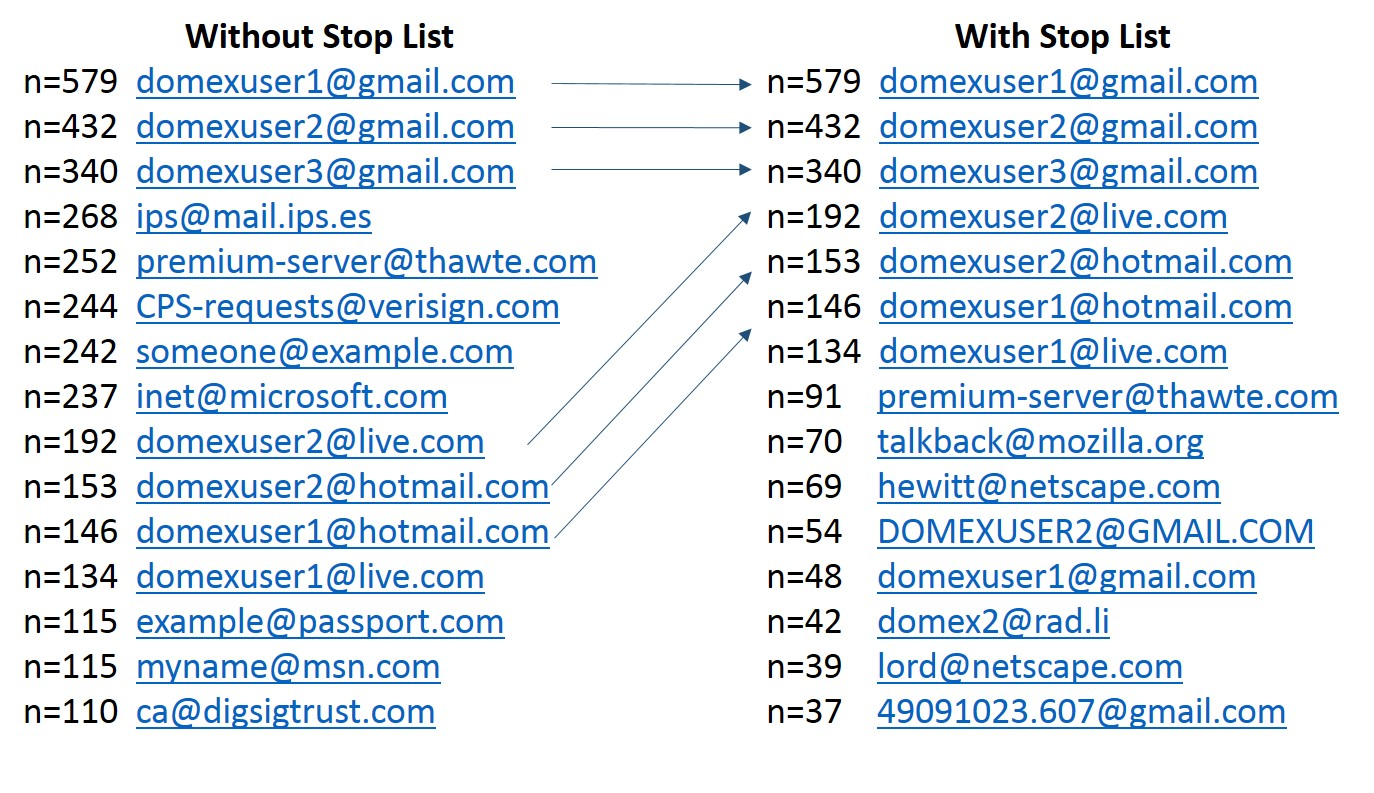
\includegraphics[scale=0.65]{otherPics/WithWithoutStopList.jpg}
	\caption{Email Histogram Results With and Without the Context-Sensitive Stop List. Results from the Domexusers HD image.}
	\label{fig:withandwithoutstoplist}
\end{figure}

It should be noted that \bulk does allow the users to create stop lists that are not context sensitive. A stop list can simply be a list of words that the user wants \bulk to ignore. For example, the following three lines would constitute a valid stop list file: 
\begin{verbatim}
abc@google.com
ignore@microsoft.com
www.google.com
\end{verbatim}

However for the reasons stated above, it is recommended that users rely on context-sensitive stop lists when available to reduce the time required to analyze the results of a \bulk run.\\

Stopped results are not completely hidden from users. If stopped feature are discovered, they will be written to the appropriate category feature file with the extension \texttt{\_stopped.txt}. For example, stopped domain names that are found in the disk image will be written to \texttt{domain\_stopped.txt} in the output directory. The stopped files serve the purpose of allowing users to verify that \bulk is functioning properly and that the lists they have written are being processed correctly.

\subsection{Using an Alert List}
Users may have specific words, or feature in a given context, that are important to their investigation. The alert list allows \bulk to specifically alert or flag the user when those concepts are found. Alert lists can contain a list of words or a feature file. The feature file operates much in the same way as the feature files used for context-sensitive stop lists. It will provide a feature but alert on that feature only when it's found in the specified context.\\

A sample alert list file might look like the following:
\begin{verbatim}
abc@google.com
SilentFury2012
www.maliciousintent.com
\end{verbatim}

While this list does not appear to help in any particular investigation, it demonstrates that you can specify distinct words that are important to their analysis. Results containing the alert list information are found in the file \texttt{alert.txt} in the run output directory.

\subsection{The Importance of Compressed Data Processing}
\label{compressedProcessing}

Many forensic tools frequently miss case-critical data because they do not examine certain classes of compressed data found. For example, a recent study of 1400 drives found thousands of email addresses that were compressed but in unallocated space\cite{encodedEvidence}. Without looking at all the data on each drive and optimistically decompressing it, those features would be missed. Compressed email addresses, such as those in a GZIP file, do not look like email addresses to a scanner; they must first be decompressed to be identified. Although some of these features are from software distributions, many are not. Table ~\ref{tab:encodings2} shows the kinds of encodings that can be decoded by \bulk \cite{encodedEvidence}.

\begin{table}[!ht]
\centering
\caption{The kinds of encodings that can be decoded by \bulk and the amount of context required for the decoding}
\label{tab:encodings2}
\begin{tabular}{|p{2 cm}|p{9 cm}|}
\hline \hline
\textbf{Encoding} & \textbf{Can be decoded when \bulk finds} \\
\hline
GZIP & The beginning of a zlib-compressed stream\\
\hline
BASE64 & The beginning of a BASE64-encoded stream \\
\hline
HIBER & Any fragment of a hibernation file can generally be decompressed, as each Windows 4k page is separately compressed and the beginning of each compressed page in the hibernation file is indicated by a well-known sequence\\
\hline
PDF & Any PDF stream compressed with ZLIB bracketed by \textit{stream} and \textit{endstream} \\
\hline
ZIP & The local file header of a ZIP-file component \\
\hline
\end{tabular}
\end{table}


The reason that users must be aware of this is because users have a tendency to want to enable and disable scanners for specific uses; They can unintentionally damage their results. For example, if a user only wants to find email addresses, they may try to turn off all scanners except the email scanner. This will find some email addresses. However, it will miss the email addresses on the media that are only present in compressed data. This is because scanners such as \textbf{\textit{zip}},  \textbf{\textit{rar}} and  \textbf{\textit{gzip}} will not be running. Those scanners each work on a different type of compressed data. For example, the  \textbf{\textit{gzip}} scanner will find GZIP compressed data, decompress it and then pass it other scanners to search for features. In that way, GZIP compressed emails can be processed by \bulk. \\

The  \textbf{\textit{pdf}} scanner is another type of scanner that finds text that otherwise wouldn't be found. While PDF files are human readable, they are not readable but many software tools and scanners because of their formatting. The  \textbf{\textit{pdf}} scanner extracts some kinds of text found within PDFs and then passes that text on to other scanners for further processing. Many typical disk images include PDF files, so most users will want to have this scanner enabled (as it is by default).\\

Finally, the  \textbf{\textit{hiber}} scanner decompresses Windows hibernation files. If the disk image being analyzed is from a Windows system, \bulk users will want that turned on (as it is by default). The scanner is very fast, however, so it will not significantly decrease performance on non-Windows drives.

\section{Use Cases for \bulk}
There are many digital forensic use cases for \bulk --- more than we can enumerate within this manual. In this section we highlight some of the most common uses of the system. Each case discusses which output files, including feature files and histograms, are most relevant to these types of investigations.  In \textbf{\Autoref{Examples}}, \textbf{\nameref{Examples}}, we provide more detailed walk-throughs and refer back to these use cases with more detailed output file information.

\subsection{Malware Investigations}
\label{malware}
Malware is a programmatic intrusion. When performing a malware investigation, users will want to look at executables, information that has been downloaded from web-based applications and windows directory entries (for Windows-specific investigations). \bulk enables this in several ways. \\

First, \bulk finds evidence of virtually all executables on the hard drive including those by themselves, those contained in ZIP files, and those that are compressed. It does not give you the hash value of the full file, rather, it gives the hash of just the first 4KB of the file. Our research has shown that the first 4KB is predictive because most executables have a distinct hash value for the first 4KB of the file \cite{hashEncoding}. Additionally, many of these files may be fragmented and looking at the first 4KB will still provide information relevant to an investigation because fragmentation is unlikely to happen before the first 4KB. The full hash of a fragmented file is not available in \bulk.\\ 

Several output feature files produced by \bulk contain relevant and important information about executables. These files include:
\begin{itemize}
\item \texttt{elf.txt} --- This file (produced by the \textbf{\textit{elf}} scanner) contains information about ELF executables that can be used to target Linux and Mac systems.
\item \texttt{winprefetch.txt} --- This file (produced by the \textbf{\textit{winprefetch} scanner} lists the current and deleted files found in the Windows prefetch directory.
\end{itemize}
The XML in these feature files is too complicated to review without using other applications. The recommended way to analyze the executable output is to use a third party tool that analyzes executables or pull the results into a spreadsheet. In a spreadsheet, one column could contain the hash values and those values can be compared against a database of executable hashes. There is also a python tool that comes with \bulk called \textbf{identify\_filenames.py} that can be used to get the full filename of the file. The python tool is discussed in more detail in \textbf{\Autoref{PostProcessing}}.\\

For Windows specific malware investigations, the files \texttt{winpe.txt} and \texttt{winprefetch.txt} are very useful. They are produced by the \textbf{\textit{winpe}} and \textbf{\textit{winprefetch}} scanners respectively.  Windows Prefetch shows files that have been prefetched in the Windows prefetch directory and shows the deleted files that were found in unallocated space. The Windows PE feature file shows entries related to the Windows executable files. \\

JSON, the JavaScript Object Notation, is a lightweight data-interchange format. Websites tend to download a lot of information using JSON. The output file \texttt{json.txt}, produced by the \textbf{\textit{json}} scanner, can be useful for malware investigations and analysis of web-based applications. If a website has downloaded information in JSON format, the JSON scanner may find that information in the browser cache. 

\subsection{Cyber Investigations}
\label{cyber}
Cyber investigations may scan a wide variety of information types. A few unifying features of these investigations are the need to find encryption keys, hash values and information about ethernet packets. \bulk provides several scanners that produce feature files containing this information.\\

For encryption information, the following feature files may be useful:
\begin{itemize}
\item \texttt{aes.txt} --- AES is an encryption system. Many implementations leave keys in memory that can be found using an algorithm invented at Princeton University. \bulk provides an improved version of that algorithm to find AES keys in the  \textbf{\textit{aes}} scanner. When it scans memory, such as swap files or decompressed hibernation files, it will identify the AES keys. The keys can be used for software that will decrypt AES encrypted material. 
\item \texttt{hex.txt} --- The  \textbf{\textit{base16}} scanner decodes information that is stored in Base16, breaking it into the corresponding hexidecimal values. This is useful if you are looking for AES keys or SHA1 hashes. This scanner only writes blocks that are of size 128 and 256 because they are the sizes used for encryption keys. The feature file is helpful if the investigator is looking for people who have emailed encryption keys or hash values in a cyber investigation.
\end{itemize}

Additionally, the  \textbf{\textit{base64}} scanner is important for cyber investigations because it looks mostly at email attachments that are coded in Base64. The information found in these attachments will be analyzed by other scanners looking for specific features.\\

The \textbf{\textit{windirs}} scanner finds Windows FAT32 and NTFS directory entries and will also be useful for cyber investigations involving Windows machines, as they may be indicators of times that activity took place.\\

Finally, the files \texttt{ether.txt}, \texttt{ip.txt}, \texttt{tcp.txt} and \texttt{domain.txt} are all produced by the  \textbf{\textit{net}} scanner. It searches for ethernet packets and memory structures associated with network data structures in memory. It is important to note that tcp connections have a lot of false positives and many of the information found by this scanner will be false. Investigators should be careful with the interpretation of these feature files for that reason.

\subsection{Identity Investigations}
\label{identity}
Identity investigations may be looking for a wide variety of information including email addresses, credit card information, telephone numbers, geographical information and keywords. For example, if the investigator is trying to find out of who a person is and who their associates are, they will be looking at phone numbers, search terms to see what they are doing and emails to see who they are communicating with. \\

The  \textbf{\textit{accts}} scanner is very useful for identity investigations. It produces several feature files with identity information including:
\begin{itemize}
\item \texttt{ccn.txt} --- credit card numbers
\item \texttt{ccn\_track2.txt} - credit card track two information -  relevant information if someone is trying to make physical fake credit cards
\item \texttt{pii.txt} - personally identifiable information including birth dates and social numbers
\item \texttt{telephone.txt} - telephone numbers
\end{itemize}

The  \textbf{\textit{kml}} and  \textbf{\textit{gps}} scanner both produce GPS information that give information about a person in a certain area or link to what they have been doing in a certain area. Both of these scanners write to \texttt{gps.txt}. KML is a format used by Google Earth and Google Map files. This scanner searches in that formatted data for GPS coordinates. The  \textbf{\textit{gps}} scanner looks at Garmin Trackpoint formatted information and finds GPS coordinates  in that data.\\

The  \textbf{\textit{email}} scanner looks for email addresses in all data and writes that to \texttt{email.txt}. The  \textbf{\textit{vcard}} scanner looks at vCard data, an electronic business card format, and finds names, email addresses and phone numbers to write to the respective feature file.\\

The are multiple url files including \texttt{url.txt}, \texttt{url\_facebook-address}, \texttt{url\_facebook-id}, \texttt{url\_microsoft-live}, \texttt{url\_searches.txt} and \texttt{url\_services.txt} that are produced by the \textbf{\textit{email}} scanner. They are useful for looking at what websites a person has visited as well as the people they are associating with.\\

An important aspect of identity investigations (as well as other types) is the ability to search the data for a list of keywords. \bulk provides the capability to do that through two different means. First, the  \textbf{\textit{find}} scanner is a simple regular expression finder that uses regular expressions. The \textbf{\textit{find}} scanner looks through the data for anything listed in the global find list. The format of the find list should be rows of regular expressions while any line beginning with a \# is considered a comment. The following is an excerpt from a sample find list file:
\lstset{style=customfile}
\begin{lstlisting}
# This is a comment line
\b\d{1,3}\.\d{1,3}\.\d{1,3}\.\d{1,3}\b
# another comment line
/^[a-z0-9_-]{3,16}$/
\end{lstlisting}
%$
The first regular expression from the above example, beginning with \texttt{\textbackslash b}, looks for the following in order: a word boundary followed a digit repeated between 1-3 times, a digit repeated between 1-3 times, a digit repeated 1-3 times, a '.', a digit repeated 1-3 times, a digit repeated 1-3 times and the end of the word boundary. That regular expression would find, for example, the sequence 2219.889 separated out from other text by a word boundary.\\

The second regular expression from the above example, beginning with \texttt{/} looks for the following in order: a '/', the beginning of a line, repeats of any character in lowercase a-z, 0-9, '\_', or '-', repeated 3 to 16 times, and the end of the line followed by '\textbackslash.' That expression would find, for example, the following sequence:
\\
\textbackslash \\
284284284284 \\
/ \\
Regular expressions can be used to represent character and number sequences (or ranges of values) that might be of particular importance to an investigation. \\

The find list is sent in as input to \bulk using the ``-F \texttt{findlist}'' option. To run \bulk with a find list, the following basic parameters are required (where \texttt{findlist.txt} is the name of the find list):
\begin{Verbatim}[commandchars=\\\{\}]
\verbbf{bulk_extractor -F findlist.txt -o output mydisk.raw}
\end{Verbatim}

Another scanner, the \textbf{\textit{lightgrep}} scanner provides the same functionality as the \textbf{\textit{find}} scanner but it is much faster and provides more functionality. It is also a regular expression scanner that looks through the buffers and matches in the global find list. A syntax sheet of regular expressions that might be helpful to users in creating a find list to be used by the Lightgrep Scanner is shown in Figure ~\ref{fig:lightgrepSyntax}. \\

\begin{figure}
	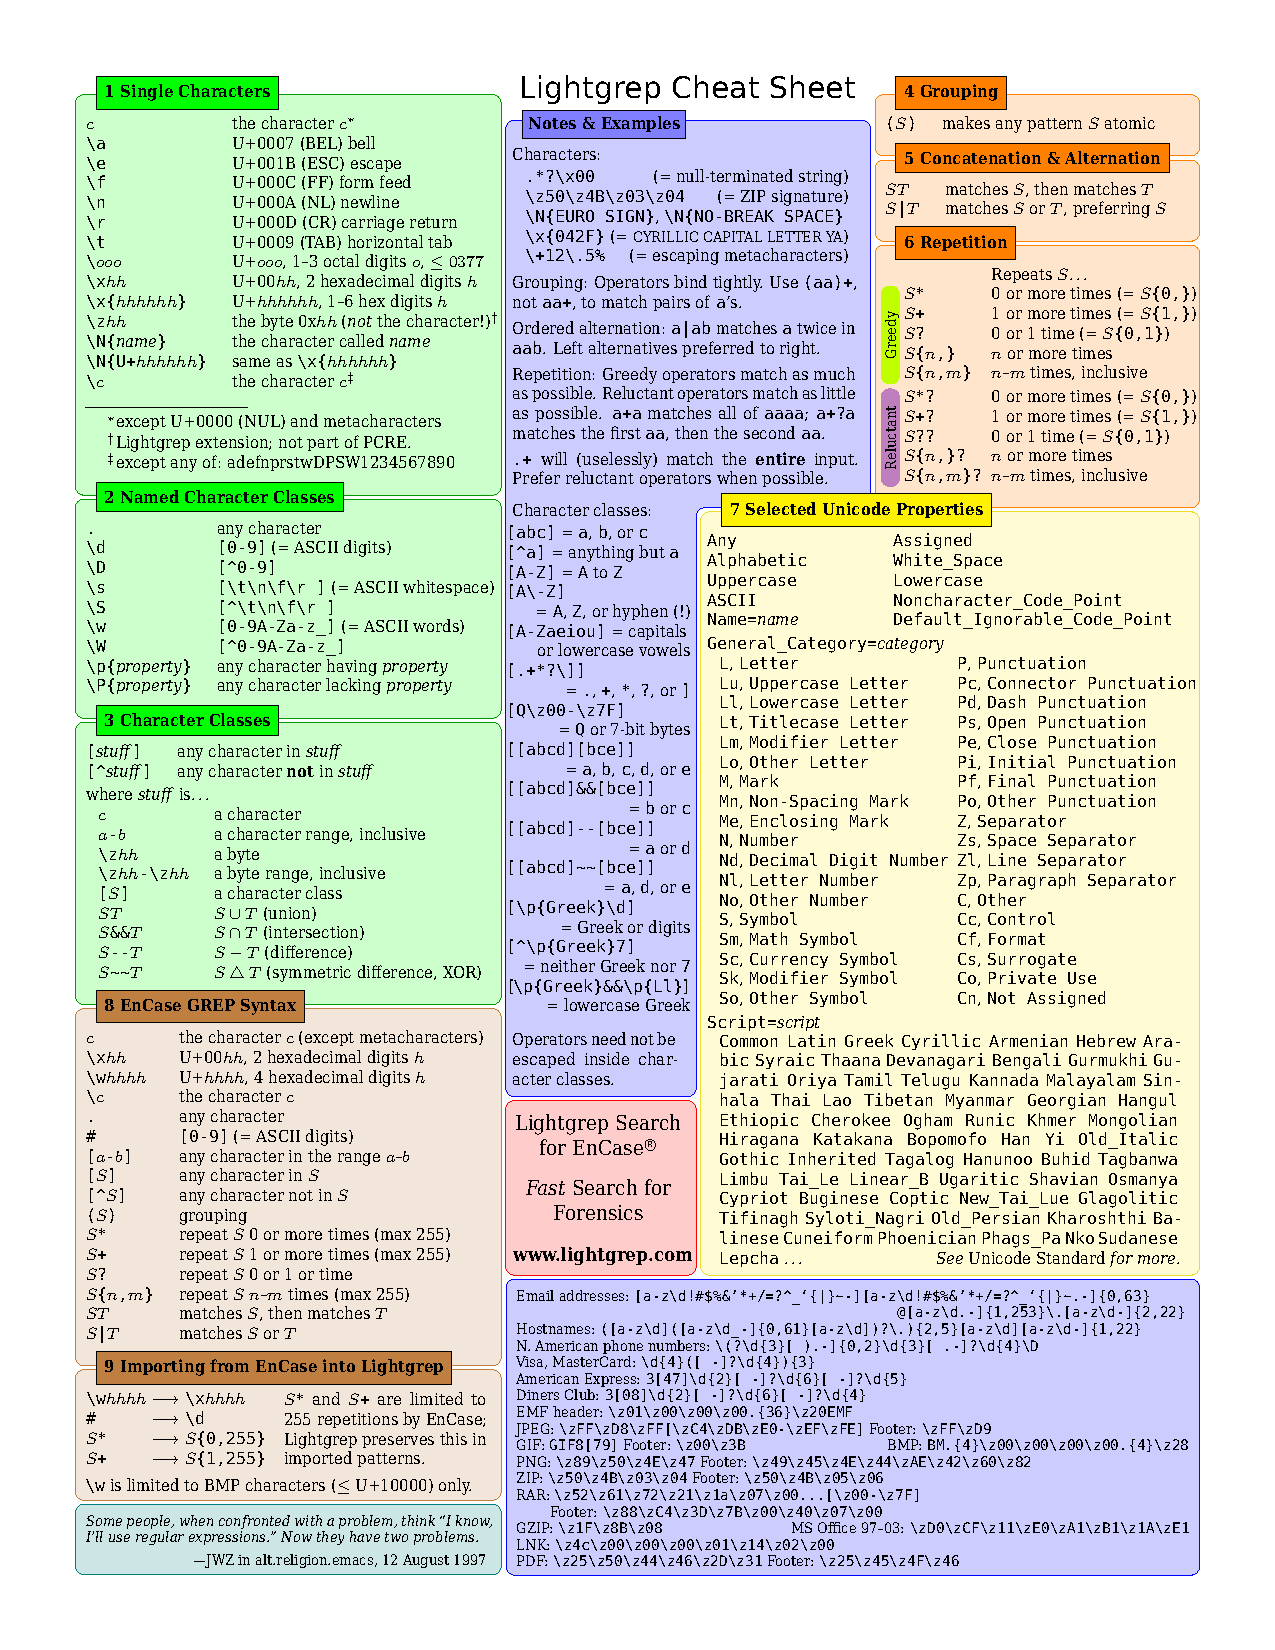
\includegraphics[scale=.80]{otherPics/LightgrepCheatSheet.pdf}
	\caption{Guide to Syntax Used by Lightgrep Scanner}
	\label{fig:lightgrepSyntax}
\end{figure}

The \textbf{\textit{lightgrep}} scanner uses the Lightgrep library from Lightbox Technologies. An open source version of that library can be downloaded from \url{https://github.com/LightboxTech/liblightgrep}. Installation instructions are also available at the download site. The \textbf{\textit{lightgrep}} scanner is preferable because it looks for all regular expressions at once, on the first pass through the data. The \textbf{\textit{find}} scanner actually looks for each expression in the find list one at a time. For example, if the find list is a list of medical terms and diagnoses and \bulk is searching medical records, the \textbf{\textit{find}} scanner looks for each term in each piece of data on one pass through, one at a time. A list of 35 expressions would require 35 passes through the data. The \textbf{\textit{lightgrep}} scanner will search a given buffer for all of the medical terms at once, in one pass through. \\

If the Lightgrep library is installed and the find list is provided to \bulk, it will run the \textbf{\textit{lightgrep}} scanner. If not, it will use the \textbf{\textit{find}} scanner. Neither scanner needs to be enabled by the user specifically, calling \bulk with the find list will automatically enable the appropriate scanner. However, we do not recommend using the find list without the Lightgrep library --- it will make \bulk run very slowly because each find search will be sequentially executed. This will provide an exponential slow-down.\\

Investigators looking for identity information may rely heavily on the find list to search for specific names, numbers or keywords relevant to the investigation. The features found by the \textbf{\textit{find}} or \textbf{\textit{lightgrep}} scanner will be written to the files \texttt{find.txt} and \texttt{lightgrep.txt} respectively.

\subsection{Password Cracking}
\label{PasswordCracking}
If an investigator is looking to crack a password, the \textbf{\textit{wordlist}} scanner can be useful. It generates a list of all the words found on the disk that are between 6 and 14 characters. Users can change the minimum and maximum size of words by specifying options at run-time but we have found this size range to be optimal for most applications. Because the \textbf{\textit{wordlist}} scanner is disabled by default, users must specifically enable it at run-time when needed. To do that, run the following command:
\begin{Verbatim}[commandchars=\\\{\}]
\verbbf{bulk_extractor -e wordlist -o output mydisk.raw}
\end{Verbatim}
This will produce two files useful for password cracking, \texttt{wordlist\_histogram.txt} and \texttt{wordlist.txt}.  These files will contain large words that can be used to recommend passwords.

\subsection{Analyzing Imagery Information}
\label{imagery}
In an investigator needs to specifically analyze imagery, for something such as a child pornography investigation, the \textbf{\textit{exif}} scanner would be useful. It finds JPEGs on the disk image and then carves the encoded ones that might be in, for example, ZIP files or hibernation files. It writes the output of this carving to \texttt{jpeg\_carved.txt}.

\subsection{Using \bulk in a Highly Specialized Environment}
If using \bulk in a specialized environment, two specific features might be useful.  The first is the option to include a banner on each output file created by \bulk. The banner file, specified in the example command below as \texttt{banner.txt} could include a security classification of the output data. When \bulk is run with the command specified below, the data in the banner file will be printed at the top of each output file produced.
\begin{Verbatim}[commandchars=\\\{\}]
\verbbf{bulk_extractor -b banner.txt -o output mydisk.raw}
\end{Verbatim}

The second feature might be useful to users in a specialized environment is the ability to develop plug-ins. Plug-ins in \bulk are external scanners that an individual or organization can run in addition to the open source capabilities provided with the \bulk system. The plug-in system gives the full power of \bulk to external developers, as all of \bulk's native scanners are written with the plug-in system. This power gives third party developers the ability to utilize proprietary or security protected algorithms and information in \bulk scanners. It is worth noting that all scanners installed with \bulk use the plug-in system, \bulk is really just a framework for running plug-ins.  The separate publication \textbf{Programmers Manual for Developing Scanner Plug-ins} \cite{programmersmanual} provides specific details on how to develop and use plug-ins with \bulk.

\section{Tuning \bulk}
All data that \bulk processes is divided into buffers called sbufs. Buffers created from disk images are created with a pre-determined size (bufsize). The buffer includes a page and an overlap area. As shown in Figure ~\ref{fig:margindepiction}, the pages overlap with each other in the red region. The red overlap region is called the margin. \bulk scans the pages one-by-one looking for features. Pages overlap with each other so that \bulk won't miss any features that cross from one page into another across boundaries.\\

Users may be looking for potentially large features that are bigger than the buffer size or that overlap into the margin. In that case, they may want to adjust the margin size or buffer size.  For example, if the input data includes a 30 MB ZIP file (possibly a software program), \bulk won't find features in the program because it overlaps the margins. To find features of that size, the margin size must be increased. \\

\begin{figure}
	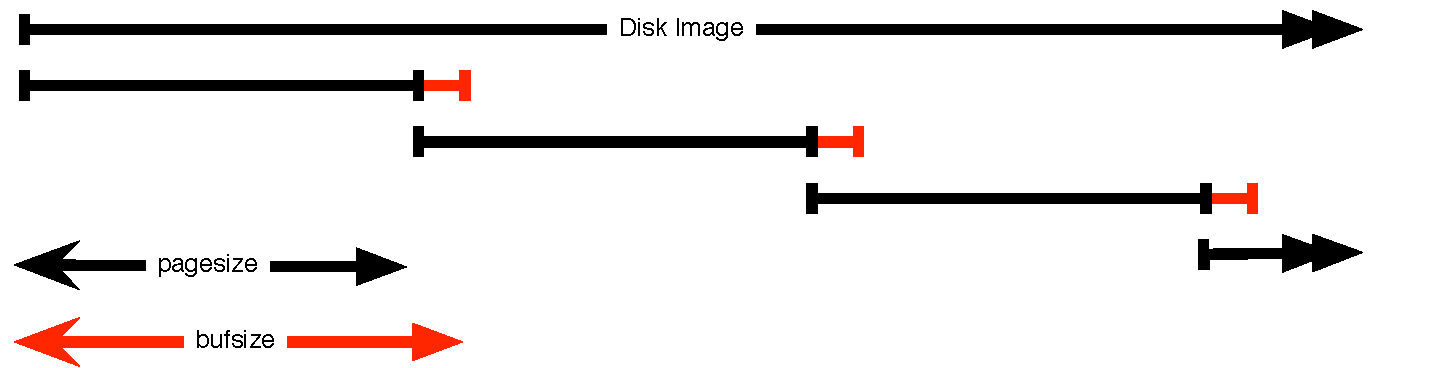
\includegraphics[scale=0.60]{archPics/margindepiction.pdf}
	\caption{Image Processor divides the disk image into buffers. Each buffer is the size of a page (\textit{pagesize}) with a buffer overlap in an area called the margin. (\textit{marginsize} is equal to \textit{bufsize-pagesize}). The buffers overlap with each other to ensure all information is processed.}
	\label{fig:margindepiction}
\end{figure}

To adjust the page size, the following usage options need to be included where NN should be set to the size (default page size is 16777216):
\begin{Verbatim}[commandchars=\\\{\}]
\verbbf{bulk_extractor -G NN -o output mydisk.raw}
\end{Verbatim}

To adjust the margin size, the following usage options need to be included where NN should be set to the size (default margin size is 4194304):
\begin{Verbatim}[commandchars=\\\{\}]
\verbbf{bulk_extractor -g NN -o output mydisk.raw}
\end{Verbatim}

\bulk provides many other tuning capabilities that are primarily recommended for users doing advanced research. Many of those options relate to specifying file sizes for input or output, specifying block sizes, dumping the contents of a buffer or ignoring certain entries. Those options are all found in the output of the -h input to \bulk and listed in \textbf{\Autoref{HelpOutput}}.

\section{Post Processing Capabilities}
\label{PostProcessing}
There are two Python programs useful for post-processing the \bulk output. Those programs are \textbf{bulk\_diff.py} and \textbf{identify\_filenames.py}. To run either of these programs, you must have Python version 2.7 or higher installed on your system. On Linux and Mac systems, the \bulk python programs are located in the directory \textit{./python} under the main \bulk installation. \\

\subsection{bulk\_diff.py: Difference Between Runs}
The program \textbf{bulk\_diff.py} takes the results of two \bulk runs and shows the differences between the two runs. This program essentially tells the difference between two disk images. It will note the different features that are found by \bulk between one image and the next. It can be used, for example, to easily tell whether or not a computer user has been visiting websites they are not supposed to by comparing a disk image from their computer from one week to the next. To run the program, users should type the following, where \textit{pre} and \textit{post} are both locations of two \bulk output directories:
\begin{Verbatim}[commandchars=\\\{\}]
\verbbf{bulk\_diff.py <pre> <post> }
\end{Verbatim} 
Note, Linux and Mac users may have to type \textbf{python2.7}, \textbf{python3}, or \textbf{python3.3} before the command, indicating the version of Python installed on your machine. An example use of the \textbf{bulk\_diff.py} program can be found in \Autoref{Examples}.


\subsection{identify\_filenames.py: Identify File Origin of Features}
The program \textbf{identify\_filenames.py} operates on the results of \bulk run and identifies the filenames (where possible) of the features that were found on the disk image. The user can run this program on one or all of the features file produced by a given run. It can be used, for example, to find the full content of an email when references to its contents are found in one of the feature files. Often email features are relevant to an investigation and an investigator would like to be able to view the full email.\\

To run this program, users will need the program \textbf{fiwalk} installed on their machine or have a DFXML file generated by \textbf{fiwalk} that corresponds to the disk image. \textbf{fiwalk} is part of the \textbf{SleuthKit} and can be installed by installing \textbf{Sleuthkit}, available at \url{http://www.sleuthkit.org/}.\\

The \textbf{identify\_filenames.py} program provides various usage options but to run the program on all feature files produced by a \bulk run, the user should type the following (where ``bulkoutputdirectory'' is the directory containing the output of a \bulk run and ``idoutput'' will contain the annotated feature files after the program runs):
\begin{Verbatim}[commandchars=\\\{\}]
\verbbf{identify\_filenames.py --all bulkoutputdirectory idoutput}
\end{Verbatim} 
Note, Linux and Mac users may have to type \textbf{python2.7}, \textbf{python3}, or \textbf{python3.3} before the command, indicating the version of Python installed on your machine.  An example use of the \textbf{bulk\_diff.py} program can be found in \Autoref{Examples}.

\section{Worked Examples}
\label{Examples}
The worked examples provided are intended to further illustrate how to use \bulk to answer specific questions and conduct investigatons. Each example uses a different, publicly available dataset and can be replicated by readers of this manual. 

\subsection {Encoding}
\newcommand\charpicture[1]{\raisebox{-2pt}[0pt][0pt]{\includegraphics[height=11pt]{#1}}}
We describe the encoding system here in order to prepare users to view
the feature files produced by \bulk. Unicode is the international
standard used by all modern computer systems to define a mapping
between information stored inside a computer and the letters, digits,
and symbols that are displayed on the screens or printed on
paper. UTF-8 is a variable width encoding that can represent every
character in the Unicode character set. It was designed for backward
compatibility with ASCII and to avoid the complications of endianness
and byte order marks in UTF-16 and UTF-32. Feature files in \bulk are
all coded in UTF-8 format. This means that the odd looking symbols,
such as accented characters (\`{e} ), funny symbols
(\charpicture{otherPics/U+2234}) and the occasional Chinese
character (\charpicture{otherPics/U+611B}) that may show up in the
files are legitimate. Glyphs from language, for example, Cyrillic
(\charpicture{otherPics/U+0428}) or Arabic (\charpicture{otherPics/U+062D}) may show up in features files as all
foreign languages can be coded in UTF-8 format. It is perfectly
appropriate and typical to open up a feature file and see characters
that the user may not recognize.\\

\section{2009-M57 Patents Scenario}
The 2009-M57-Patents scenario tracks the first four weeks of corporate history of the (fictional) M57 Patents company. The company started operation on Friday, November 13th, 2009, and ceased operation on Saturday, December 12, 2009. This specific scenario was built to be used as a teaching tool both as a disk forensics exercise and as a network forensics exercise. The scenario data is also useful for computer forensics research because the hard drive of each computer and each computers memory were imaged every day. In this example, we are not particularly interested in the exercises related to illegal activity, exfiltration and eavesdropping; they do however provide interesting components for us to examine in the example data\cite{m57scenario}.

\subsection{Run \bulk with the Data}
For this example, we downloaded and utilized one of the disk images from the 2009-M57-Patents Scenario. Those images are available at \url{http://digitalcorpora.org/corp/nps/scenarios/2009-m57-patents/drives-redacted/}. The file used throughout this example is called \texttt{charlie-2009-12-11.E01}. Running \bulk on the command line produces the following output (text input by the user is bold):\\

\begingroup
\footnotesize
\texttt{C:\textbackslash bulk\_extractor\textgreater \textbf{bulk\_extractor -o ../Output/charlie-2009-12-11 charlie-2009-12-11.E01}}
\endgroup
\begingroup
\footnotesize
\begin{Verbatim}[fontfamily=courier, commandchars=\\\{\}]
bulk_extractor version: 1.4.0
Input file: charlie-2009-12-11.E01
Output directory: ../Output/charlie-2009-12-11
Disk Size: 10239860736
Threads: 4
 8:02:08 Offset 67MB (0.66%) Done in  1:21:23 at 09:23:31
 8:02:34 Offset 150MB (1.47%) Done in  1:05:18 at 09:07:52
 8:03:03 Offset 234MB (2.29%) Done in  1:01:39 at 09:04:42
 8:03:49 Offset 318MB (3.11%) Done in  1:09:19 at 09:13:08
...
9:06:23 Offset 10049MB (98.14%) Done in  0:01:13 at 09:07:36
9:06:59 Offset 10133MB (98.96%) Done in  0:00:41 at 09:07:40
9:07:29 Offset 10217MB (99.78%) Done in  0:00:08 at 09:07:37

All data are read; waiting for threads to finish...
Time elapsed waiting for 4 threads to finish:
     (timeout in 60 min .)
Time elapsed waiting for 3 threads to finish:
    7 sec (timeout in 59 min 53 sec.)
Thread 0: Processing 10200547328
Thread 2: Processing 10217324544
Thread 3: Processing 10234101760

Time elapsed waiting for 2 threads to finish:
    13 sec (timeout in 59 min 47 sec.)
Thread 0: Processing 10200547328
Thread 2: Processing 10217324544

All Threads Finished!
Producer time spent waiting: 3645.8 sec.
Average consumer time spent waiting: 3.67321 sec.
*******************************************
** bulk_extractor is probably CPU bound. **
**    Run on a computer with more cores  **
**      to get better performance.       **
*******************************************
Phase 2. Shutting down scanners
Phase 3. Creating Histograms
   ccn histogram...   ccn_track2 histogram...   domain histogram...
   email histogram...   ether histogram...   find histogram...
   ip histogram...   lightgrep histogram...   tcp histogram...
   telephone histogram...   url histogram...   url microsoft-live...
   url services...   url facebook-address...   url facebook-id...
   url searches...Elapsed time: 3991.77 sec.
Overall performance: 2.56524 MBytes/sec
Total email features found: 15277
\end{Verbatim}
\endgroup
\begin{figure}
	\center
	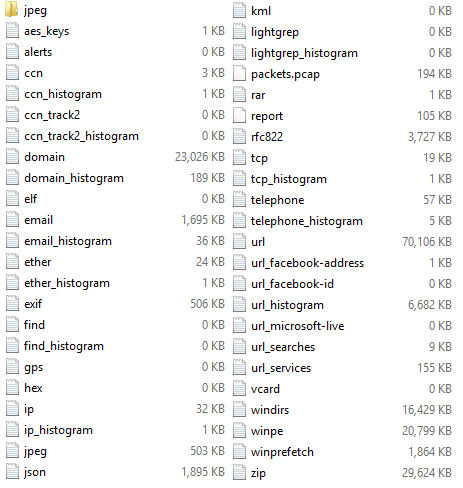
\includegraphics[scale=1.00]{charlieRunOutput.png}
	\caption{Screenshot from Windows Explorer of the Output Directory Created by the \bulk run}
	\label{fig:charlieOutput}
\end{figure}
All of the results from the \bulk run are stored in the output directory \textit{charlie-2009-12-11}. The contents of that directory after the run include the feature files, histogram files and carved output. Figure ~\ref{fig:charlieOutput} is a screenshot of the Windows output directory. Additionally, the following output shows a list of the files, directories and their sizes under Linux:

\begingroup
\footnotesize
\texttt{C:\textbackslash bulk\_extractor\textbackslash charlie-2009-12-11\textgreater \textbf{ls -s -F}}
\endgroup
\begingroup
\footnotesize
\begin{Verbatim}[fontfamily=courier, commandchars=\\\{\}]
    1 aes_keys.txt                  0 kml.txt
    0 alerts.txt                    0 lightgrep.txt
    4 ccn.txt                       0 lightgrep_histogram.txt
    1 ccn_histogram.txt           196 packets.pcap
    0 ccn_track2.txt                1 rar.txt
    0 ccn_track2_histogram.txt    108 report.xml
23028 domain.txt                 3728 rfc822.txt
  192 domain_histogram.txt         20 tcp.txt
    0 elf.txt                       4 tcp_histogram.txt
 1696 email.txt                    60 telephone.txt
   36 email_histogram.txt           8 telephone_histogram.txt
   24 ether.txt                 70108 url.txt
    1 ether_histogram.txt           1 url_facebook-address.txt
  508 exif.txt                      0 url_facebook-id.txt
    0 find.txt                   6684 url_histogram.txt
    0 find_histogram.txt            0 url_microsoft-live.txt
    0 gps.txt                      12 url_searches.txt
    0 hex.txt                     156 url_services.txt
   32 ip.txt                        0 vcard.txt
    4 ip_histogram.txt          16432 windirs.txt
   12 jpeg/                     20800 winpe.txt
  504 jpeg.txt                   1864 winprefetch.txt
 1896 json.txt                  29624 zip.txt
\end{Verbatim}
\endgroup
Many of the feature files and histograms are populated with data. Additionally, there were some JPEG files carved and placed in the \textit{jpeg} directory. In the following sections, we demonstrate how to look at these results to discover more information about the disk user and the files contained on the disk image.

\subsection{Digital Media Triage}
Digital media triage is the process of using the results of a rapid and automated analysis of the media, performed when the media is first encountered to determine if the media is likely to have information of intelligence value and, therefore, should be prioritized for immediate analysis. \bulk performs bulk data analysis to help investigators quickly decide which piece of digital media is the most relevant and useful to an investigation. Thus, \bulk can be used to aid in investigations (through the identification of new leads and social networks) rather than just aiding in conviction-support (through the identification of illegal materials)\cite{digitalmediatriage}.\\

In this example, we look at the \texttt{charlie-2009-12-11.E01} image to quickly assess what kinds of information useful to an investigation might be present on the disk. For the purposes of this example, we will assume we are investigating corporate fraud and trying to discover the answers to the following questions:
\begin{itemize}
\item Who are the users of the drive?
\item Who is this person communicating with?
\item What kinds of websites have they have been visiting most often?
\item What search terms are used?
\end{itemize}

To answer many of these questions, we look at the identify information on the drive including email addresses, credit card information, search terms, Facebook IDs, domain names and vCard data. The output files created by \bulk contain all of this type of information that was found on the disk image. \\

The scenario setup leads us to believe that Charlie is the user of the this drive (based on the name of the disk image). First, we look at \texttt{email.txt} to find information about the email addresses contained on the disk. The first two lines of the email features found are the following (each block of text represents one long line of offset, feature and context):
\lstset{style=customfile}
\begin{lstlisting}
50395384	n\x00o\x00m\x00b\x00r\x00e\x00_\x001\x002\x003\x00@\x00h\x00o\x00t
\x00m\x00a\x00i\x00l\x00.\x00c\x00o\x00m\x00    e\x00m\x00p\x00l\x00o\x00\x00\x0A\x00
\x09\x00n\x00o\x00m\x00b\x00r\x00e\x00_\x001\x002\x003\x00@\x00h\x00o\x00t\x00m
\x00a\x00i\x00l\x00.\x00c\x00o\x00m\x00\x0A\x00\x09\x00m\x00i\x00n\x00o\x00m\x00b\x00

50395432	m\x00i\x00n\x00o\x00m\x00b\x00r\x00e\x00@\x00m\x00s\x00n\x00.\x00c
\x00o\x00m\x00	i\x00l\x00.\x00c\x00o\x00m\x00\x0A\x00\x09\x00m\x00i\x00n\x00o\x00m
\x00b \x00r\x00e\x00@\x00m\x00s\x00n\x00.\x00c\x00o\x00m\x00\x0A\x00\x09\x00e\x00j
\x00e\x00m\x00p\x00l\x00
\end{lstlisting}

It is important to note that UTF-16 formatted text is escaped with \textbackslash x00. This means that "\textbackslash x00t \textbackslash x00e \textbackslash x00x \textbackslash x00t" translates to "text." The first two features found are "nombre\_123@hotmail.com" and "minombre@msn.com."  Both of the offset values, 50395384 and 50395432, are early on the disk. At this point, there is no way to know if either of these email addresses are of any significance unless they happen to belong to a suspect or person related to the investigation. The first set of email features found appear on the disk printed in UTF-16 formatted text, like the lines above.\\

Further down in the feature file, we find the following:
\lstset{style=customfile}
\begin{lstlisting}
9263459	charlie@m57.biz	21)(88=Charlie <charlie@m57.biz>)(89\x0D\x0A    =Pat 
9263497	pat@m57.biz	    =Pat McGoo <pat@m57.biz>)(8B=WELCOME TO
\end{lstlisting}

Finding Charlie's email address on the computer begins to further confirm the assumption that this is his computer. The \texttt{email\_histogram.txt} file provides important information. It shows the most frequently occurring email addresses found on the disk. The following is an excerpt from that top of that file:
\lstset{style=customfile}
\begin{lstlisting}
n=875	mozilla@kewis.ch	(utf16=3)
n=651	charlie@m57.biz	(utf16=120)
n=605	ajbanck@planet.nl
n=411	mikep@oeone.com
n=395	belhaire@ief.u-psud.fr
n=379	premium-server@thawte.com	(utf16=11)
n=356	lilmatt@mozilla.com
n=312	cedric.corazza@wanadoo.fr
\end{lstlisting}
This histogram output shows us that Charlie's email address is the second most frequently occurring name on the disk. It would likely be the first but, as described in the scenario description, this company has only been in business for three weeks and its employees are new users of the computers. Looking at this histogram file also gives us some insight into who the user of this disk is communicating with. Those email addresses occurring most frequently that are not part of the software installed on the machine (such as ajbanck@planet.nl) might indicate addresses of people with whom the drive user is corresponding or they may result from other software or web pages that were downloaded. (In this case, the email is from a Firefox extension.)\\

The file \texttt{domain.txt} provides a list of all the "domains" and host names that were found. The sources include URLS, email and dotted quads. Much of the beginning of the feature file is populated with microsoft.com domains. This is largely due to the fact that the disk image is from a Windows machine. Further down in the file we find the following:
\lstset{style=customfile}
\begin{lstlisting}
53878576	www.uspto.gov	<a href="http://www.uspto.gov/patft/index.htm
53879083	www.uspto.gov	<A HREF="http://www.uspto.gov/patft/help/help
53880076	ebiz1.uspto.gov	<A HREF="http://ebiz1.uspto.gov/vision-service/
53880536	ebiz1.uspto.gov	<A HREF="http://ebiz1.uspto.gov/vision-service/
\end{lstlisting}

The domains that were found make sense given that the disk image was obtained from a startup company that deals with patents. Many of the domains found in the file are also in UTF-16 format (with "escaped" characters). It is also worth noting as users browse the domain output file that domains are common in compressed data.\\

The \texttt{domain\_histogram.txt} file provides a histogram of the domains found on the disk image. It tends to give us better information for digital media triage than the \texttt{domain.txt} file as it provides information about which domains most frequently appear on the disk image and not just the order in which they were found. The beginning of the histogram file looks like the following:
\lstset{style=customfile}
\begin{lstlisting}
n=10749	www.w3.org
n=6670	chroniclingamerica.loc.gov
n=6384	openoffice.org
n=5998	www.uspto.gov
n=5733	www.mozilla.org
n=5212	www.osti.gov
n=4952	www.microsoft.com
n=4470	patft.uspto.gov
\end{lstlisting}

Many of these domains are part of the operating system, such as openoffice.org, but some are not, such as www.uspto.gov. The histogram file provides insight into the users activity on the machine and which sites they were most frequently visiting. \\

The file \texttt{rfc822.txt} primarily provides email headers and HTTP headers both of which are in a format specified by RFC822, the Internet Message Standard. It can be useful to see the subject of emails that have been sent and information form HTTP requests. The following is an excerpt from the text file:
\lstset{style=customfile}
\begin{lstlisting}
114074196 SUBJECT:softabs	ll|micro)\x5CW?cap\x00SUBJECT:softabs\x00SUBJECT:Caili
114074212 SUBJECT:Cailis	SUBJECT:softabs\x00SUBJECT:Cailis\x00\x00SUBJECT:st0ck
114074228 SUBJECT:st0ck	SUBJECT:Cailis\x00\x00SUBJECT:st0ck\x00\x00\x00SUBJECT:Your 
114074244 SUBJECT:Your Personal Quarantine Folder
SUBJECT:st0ck\x00\x00\x00SUBJECT:Your Personal Quarantine Folder\x00SUBJECT:rolex\x00
114074284	SUBJECT:rolex arantine Folder\x00SUBJECT:rolex\x00\x00\x00SUBJECT:(bro
\end{lstlisting}
Much of what is found in the file shown above are spam messages.\\

Telephone numbers found on the disk image are stored in \texttt{telephone.txt}. This following numbers found in the file are clearly for technical support (found within installed software):
\lstset{style=customfile}
\begin{lstlisting}
88850883 (800) 563-9048 rmation centre: (800) 563-9048\x0D\x0A<BR><b><i>Tech
88850995 (905) 568-4494 indows&nbsp;95: (905) 568-4494\x0D\x0A<BR> Microsoft
88851056 (905) 568-2294 ice components: (905) 568-2294\x0D\x0A<BR> Other sta
88851111 (905) 568-3503 hnical support: (905) 568-3503\x0D\x0A<BR> Priority 
88851162 (800) 668-7975 rt information: (800) 668-7975\x0D\x0A<BR> Text Tele
\end{lstlisting}
The next set of "telephone" numbers are clearly bogus numbers:
\lstset{style=customfile}
\begin{lstlisting}
3649684174 008-017-0108 WA,98366,1,4031-008-017-0108,City of Port Or
3649684741 000-031-0009 98337,0.13,3768-000-031-0009,Kitsap County C
3649818237 000-001-0005 8312,2.25,"3768-000-001-0005, 3768-000-003-0
3649818274 000-004-0002 0-003-003, 3768-000-004-0002, 3768-000-005-0
\end{lstlisting}
Finally, many of the numbers found are legitimate ones. These numbers were all found in GZIP compressed data:
\lstset{style=customfile}
\begin{lstlisting}
3772517888-GZIP-28322 (831) 373-5555 onterey - <nobr>(831) 373-5555</nobr><br><a cl
3772517888-GZIP-29518 (831) 899-8300 Seaside - <nobr>(831) 899-8300</nobr><br><a cl
3772517888-GZIP-31176 (831) 899-8300 Seaside - <nobr>(831) 899-8300</nobr><br><a cl
\end{lstlisting}
Typically, the file \texttt{telephone\_histogram.txt} is the best place to look for phone numbers. In this file, the non-digits are extracted from the phone numbers. The following is an excerpt from the beginning of that file:
\lstset{style=customfile}
\begin{lstlisting}
n=42	+14159618830
n=35	8477180400
n=24	+27112570000
n=24	2225552222
n=18	8005043248
n=15	2225551111
n=13	8662347350
n=12	8772768437
n=11	2522277013
\end{lstlisting}
Investigators looking for specific information about the user of a disk image or who they have been communicating with can look quickly at this file and see how frequently numbers appear. It also consolidates the numbers in a way that makes it easy for investigators looking for a specific number or set of numbers to see them quickly.\\

Finally, in performing digital media triage on the disk image, investigators would like to know what specific URLs have been visited and what search terms the user has been using. The set of URL files provided as output provide insight into this information. First, \texttt{url.txt} contains the URLs found on the disk. The following is an excerpt from that file (note that the UTF-16 formatted information is escaped):
\lstset{style=customfile}
\begin{lstlisting} 
175165385 http://www.unicode.org/reports/tr25/#_TocDelimiters E and U+23DF:\x0A#
http://www.unicode.org/reports/tr25/#_TocDelimiters\x0A\x5Cu23DE = \x5CuE13B

159045397 h\x00t\x00t\x00p\x00:\x00/\x00/\x00w\x00w\x00w\x00.\x00d\x00o\x00w
\x00n\x00l\x00o\x00a\x00d\x00.\x00w\x00i\x00n\x00d\x00o\x00w\x00s\x00u\x00p
\x00d\x00a\x00t\x00e\x00.\x00c\x00o\x00m\x00/\x00m\x00s\x00d\x00o\x00w\x00n\x00l\x00o
\x00a\x00d\x00/\x00u\x00p\x00d\x00a\x00t\x00e\x00/\x00s\x00o\x00f\x00t\x00w\x00a\x00r
\x00e\x00/\x00s\x00e\x00c\x00u\x00/\x002\x000\x000\x008\x00/\x000\x006\x00/\x00w\x00i
\x00n\x00d\x00o\x00w\x00s\x00x\x00p\x00-\x00k\x00b\x009\x005\x001\x003\x007\x006\x00-
\x00v\x002\x00-\x00x\x008\x006\x00-\x00e\x00n\x00u\x00_\x00e\x009\x00b\x006\x008\x00c
\x005\x00e\x006\x003\x00a\x00c\x00b\x005\x007\x008\x006\x00a\x000\x005\x00b\x005\x003
\x00b\x004\x00 \xB4\xF4\x82\x94C\xE3\xB6C\xB1p\x9Ae\xBC\x82,wh\x00t\x00t\x00p\x00:
\x00/\x00/\x00w\x00w\x00w\x00.\x00d\x00o\x00w\x00n\x00l\x00o\x00a\x00d\x00.\x00w
\x00i\x00n\x00d\x00o\x00w\x00s\x00u\x00p\x00d\x00a\x00t\x00e\x00.\x00c\x00o
\x00m\x00/\x00m\x00s\x00d\x00o\x00w\x00n\x00l\x00o\x00a\x00d\x00/\x00u\x00p\x00d
\x00a\x00t\x00e\x00/\x00s\x00o\x00f\x00t\x00w\x00a\x00r\x00e\x00/\x00s\x00e\x00c\x00u
\x00/\x002\x000\x000\x008\x00/\x000\x006\x00/\x00w\x00i\x00n\x00d\x00o\x00w\x00s\x00x
\x00p\x00-\x00k\x00b\x009\x005\x001\x003\x007\x006\x00-\x00v\x002\x00-\x00x\x008\x006
\x00-\x00e\x00n\x00u\x00_\x00e\x009\x00b\x006\x008\x00c\x005\x00e\x006\x003\x00a\x00c
\x00b\x005\x007\x008\x006\x00a\x000\x005\x00b\x005\x003\x00b\x004\x003\x003\x002\x004
\x006\x005\x00d\x00e\x00

175197993	http://www.uspto.gov/patft/index.html enter>\x0A<a href="http://www.
uspto.gov/patft/index.html"><img src="/net

175198500	http://www.uspto.gov/patft/help/help.htm e></a>\x0A<AHREF="http://www.
uspto.gov/patft/help/help.htm"><IMG BORDER="0
\end{lstlisting}
The file \texttt{url\_histogram.txt} provides the histogram of the potential urls. In that file, UTF-16 formatted text is converted to UTF-8. Note that not all URLs contained in the histogram file are accurate. The are actually URLs that were typed into a web browser. The following are lines taken from that file:
\lstset{style=customfile}
\begin{lstlisting}
n=3922	http://www.mozilla.org/keymaster/gatekeeper/there.is.only.xul	(utf16=2609)
n=859	http://www.mozilla.org/keymaster/gatekeeper/there.is.only.xu	(utf16=858)
...
n=2	http://math.nist.gov/~KRemington/papers/europvm.ps
n=2	http://math.nist.gov/~MDonahue/pubs/nan.ps.gz
n=2	http://math.nist.gov/~RBoisvert/publications/ADL95.ps.gz
n=2	http://math.nist.gov/~RBoisvert/publications/IMACS97.ps.gz
\end{lstlisting}
Because the histogram file converts the UT-16 formatted text to UTF-8, the histogram file is more human readable than the \texttt{url.txt} file alone. The files \texttt{url\_facebook.txt}, \texttt{url\_microsoft-live}, \texttt{url\_services} and \texttt{url\_searches} all extract specific types of information from URLs. The most useful for digital media triage is likely the file \texttt{url\_searches.txt} because it shows histogram of searches from the disk image. Searches frequently convey intent. The following is an excerpt from that file:
\lstset{style=customfile}
\begin{lstlisting}
n=60	1
n=53	exotic+car+dealer
n=41	ford+car+dealer
n=34	2009+Shelby
n=25	steganography
n=23	General+Electric
n=23	time+travel
n=19	steganography+tool+free
n=19	vacation+packages
n=16	firefox
n=16	quicktime
n=14	7zip
\end{lstlisting}


The file \texttt{ccn.txt} provides credit card numbers that have been found on the disk. Based on the scenario set-up for this disk image, credit card numbers are not necessarily highly relevant to this investigation. However, \bulk did find some credit card numbers on this disk image that are not actually credit card numbers; This is common behavior so it is worth examining the file here to demonstrate how it can be used in other investigations. The credit card number finder considers a pattern of digits and uses the Luhn checksum algorithm and the distribution of digits and the local context to identify potential credit card numbers. It is important to note that there are frequently false positives. The first few lines of the \texttt{ccn.txt} file for this disk image look like the following:
\lstset{style=customfile}
\begin{lstlisting}
88284672-GZIP-177427 5273347458642687 734B55CD5\x0A5273347458642687\x0AC0841BAFA1B4C28
4814857216-GZIP-793 4015751530102097 ebO.d=0;ebO.rnd=4015751530102097;ebO.title="";eb
4909069775 6543210123456788	\x0Addadd7540 add '6543210123456788' 0.499999999   
4909069811 6543210123456788 499999999   -> '6543210123456788' Inexact Rounde
4909069861 6543210123456788 \x0Addadd7541 add '6543210123456788' 0.5           
4909069897 6543210123456788 5           -> '6543210123456788' Inexact Rounde
4909069947 6543210123456788 \x0Addadd7542 add '6543210123456788' 0.500000001   
5304221350 5678901234560000 +4   -> 5678901234560000\x0D\x0Addshi052 shift
5612375618 6543210123456788 \x0D\x0Aaddx6240 add '6543210123456788' 0.499999999   
5612375654 6543210123456788 499999999   -> '6543210123456788' Inexact Rounde
5612375703 6543210123456788 \x0D\x0Aaddx6241 add '6543210123456788' 0.5           
5612375739 6543210123456788 5 -> '6543210123456788' Inexact Rounde
5612375788 6543210123456788 \x0D\x0Aaddx6242 add '6543210123456788' 0.500000001   
5612715901 5700122152274696 div4036 divide  5700122152274696   5700122152251
\end{lstlisting}
In the above example, `525273347458642687' looks like it could be a valid credit card number from the context (\textbackslash x0A is a new line). The number `4015751530102097' looks like a random number in a piece of Java Script. Note that both of those numbers were compressed; the offset indicates they were found in GZIP streams (shown as a number followed by `-GZIP'). The numbers whose context include ``Inexact Rounde'' are actually from Python source code and not credit card numbers at all. Again, the \texttt{ccn.txt} tends to alert on a lot of false positives. \\ 

The \texttt{ccn\_track2.txt} file did not find any information in this disk image but is also useful for credit card fraud and identity theft investigations. It will contain credit card track 2 information found on the disk image.\\

Using the files produced by \bulk described above, an investigator can quickly review a disk image for important information that is relevant to an investigation and find actionable intelligence quickly. 

\subsection{Analyzing Imagery} 
The scenario described in the M57 Patents data is not necessarily relevant to an imagery investigation. However, there is imagery information on the disk. We use that information here to demonstrate how imagery information can be analyzed by an investigator using \bulk.\\

The file in the output directory, \texttt{jpeg.txt}, lists all JPEGs that were found on the disk whether they were carved or not. \bulk was run with default values meaning that only encoded JPEGs were carved. The following excerpt from the JPEG file shows information about JPEGs found on the disk image:
\lstset{style=customfile}
\begin{lstlisting}
54798824	../Output/charlie-2009-12-11/jpeg/54783488.jpg	<fileobject><filename>
../Output/charlie-2009-12-11/jpeg/54783488.jpg</filename><filesize>15336</filesize>
<hashdigest type='md5'>13823ce7c21587d31f6eb4474612e660
</hashdigest></fileobject>
\end{lstlisting}
The JPEG described above was not carved because it was not encoded. However, the first section ``../Output/charlie-2009-12-11/jpeg/54783488.jpg'' shows where the file would be found in the output directories if it had been carved. The next section of information also gives the file size, the hash type (in this case `md5') and the hash value of the file (in this case 13823ce7c21587d31f6eb4474612e660). Note that this may not match the hash value of the file in the original file system as \bulk cannot properly carve fragmented files.\\

Information about encoded JPEGs can also be found in the \texttt{jpeg.txt} file. The following excerpt shows a description of a JPEG found in a GZIP format on the disk:
\lstset{style=customfile}
\begin{lstlisting}
3771686400-GZIP-8332	../Output/charlie-2009-12-11/jpeg/3771686400-GZIP-0.jpg
<fileobject><filename>../Output/charlie-2009-12-11/jpeg/3771686400-GZIP-0.jpg
</filename><filesize>8332</filesize><hashdigest type='md5'>
5b77035c983b04996774370f735ea72a</hashdigest></fileobject>
\end{lstlisting}
The JPEG described above was carved and can be found in the \textit{/jpeg} output directory in the file named \texttt{3771686400-GZIP-0.jpg}. The file also gives information about the filesize, hash type and hash ID. That file is shown in the  directory output shown below along with all of the encoded JPEGs that were found on the disk image and were carved. The contents of the \textit{/jpeg} directory are as follows:

\begingroup
\footnotesize
\begin{Verbatim} 
10037939712-GZIP-0.jpg  5324841013-ZIP-0.jpg
10117679783-ZIP-0.jpg   6039195136-GZIP-0.jpg
3761630720-GZIP-0.jpg   6039215616-GZIP-0.jpg
3764534784-GZIP-0.jpg   6039223808-GZIP-0.jpg
3771686400-GZIP-0.jpg   6039232000-GZIP-0.jpg
3771706880-GZIP-0.jpg   6039244288-GZIP-0.jpg
3771715072-GZIP-0.jpg   6039301632-GZIP-0.jpg
3771723264-GZIP-0.jpg   6039318016-GZIP-0.jpg
3771735552-GZIP-0.jpg   6883925636-ZIP-0.jpg
3771792896-GZIP-0.jpg   6884040324-ZIP-0.jpg
3771809280-GZIP-0.jpg   6884056948-ZIP-0.jpg
3771833856-GZIP-0.jpg   7276064256-GZIP-0.jpg
3771858432-GZIP-0.jpg   7279128576-GZIP-0.jpg
429788672-GZIP-0.jpg    8877243047-ZIP-0.jpg
5310405287-ZIP-0.jpg    9948655104-GZIP-0.jpg
\end{Verbatim}
\endgroup
All of these JPEG files can be viewed and used by investigators. The filename is the forensic path of where the JPEG was found. The file \texttt{3771686400-GZIP-0.jpg} mentioned above is shown in Figure ~\ref{fig:carvedJPEG}.

\begin{figure}
	\center
	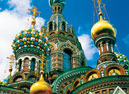
\includegraphics[scale=.90]{carvedJPEG.jpg}
	\caption{A JPEG carved from encoded data on the M57 Patents disk image}
	\label{fig:carvedJPEG}
\end{figure}

\subsection{Password Cracking}
The \textbf{\textit{wordlist}} generates a list of all the words found on the disk that are between 6 and 14 characters long. The word list that is generated by the scanner can be very useful in determining combinations of words to use for password cracking. The scanner is enabled by default because it slows down the \bulk run significantly.  To show the word list in this example, \bulk was run again on the M57 Patents scenario data with the \textbf{\textit{wordlist}} scanner enabled. Running \bulk on the command line with it enabled produces the following output:


\begingroup
\footnotesize
\texttt{C:\textbackslash be\textbackslash \textgreater \textbf{bulk\_extractor -e wordlist -o ../Output/charlie-wordlist charlie-2009-12-11.E01}}
\endgroup
\begingroup
\footnotesize
\begin{Verbatim}[fontfamily=courier, commandchars=\\\{\}]
bulk_extractor version: 1.4.0
Input file: charlie-2009-12-11.E01
Output directory: ../Output/charlie-wordlist
Disk Size: 10239860736
Threads: 4
12:58:46 Offset 67MB (0.66%) Done in  1:14:55 at 14:13:41
...
14:03:24 Offset 10217MB (99.78%) Done in  0:00:08 at 14:03:32
All data are read; waiting for threads to finish...
Time elapsed waiting for 4 threads to finish:
     (timeout in 60 min .)
Time elapsed waiting for 4 threads to finish:
    8 sec (timeout in 59 min 52 sec.)
Thread 0: Processing 10200547328
Thread 1: Processing 10234101760
Thread 2: Processing 10183770112
Thread 3: Processing 10217324544

Time elapsed waiting for 1 thread to finish:
    14 sec (timeout in 59 min 46 sec.)
Thread 3: Processing 10217324544

All Threads Finished!
Producer time spent waiting: 3627.92 sec.
Average consumer time spent waiting: 4.1518 sec.
*******************************************
** bulk_extractor is probably CPU bound. **
**    Run on a computer with more cores  **
**      to get better performance.       **
*******************************************
Phase 2. Shutting down scanners
Phase 3. Uniquifying and recombining wordlist
Phase 3. Creating Histograms
   ccn histogram...   ccn_track2 histogram...   domain histogram...
   email histogram...   ether histogram...   find histogram...
   ip histogram...   lightgrep histogram...   tcp histogram...
   telephone histogram...   url histogram...   url microsoft-live...
   url services...   url facebook-address...   url facebook-id
   url searches...Elapsed time: 4065.09 sec.
Overall performance: 2.51898 MBytes/sec
Total email features found: 152775
\end{Verbatim}
\endgroup

Note that it took 3991.71 seconds to run \bulk without the \textbf{\textit{wordlist}} scanner enabled and, in this case, it took 4065.09 seconds with \textbf{\textit{wordlist}} enabled.  The new output directory contains a file called \texttt{wordlist.txt}. That file has both filenames and words in it. The following is an excerpt from that file:
\lstset{style=customfile}
\begin{lstlisting}
50497556	usemodem.jpg
50497624	usemsn.jpg
50497692	usemsnnow.jpg
50497760	welcome.htm
50497828	whereNow.htm
50497896	xmlutil.js
50497987	^Photoshop
50498009	Resolution
50498050	Global
50498057	Lighting
50498090	Global
50498097	Altitude
50498153	Copyright
50498181	Japanese
50498229	Halftone
50498238	Settings
50498335	Transfer
\end{lstlisting}
The wordlist contains ALL words found on the disk between 6 and 14 characters long. Automated programs can be used to generate passwords from combinations of these words. The \textbf{\textit{wordlist}} scanner also generates a split wordlist containing the same words found in the \texttt{wordlist.txt} file with all words deduplicated, sorted by size and alphabetized. The following is an excerpt from the file \texttt{wordlist\_split\_000.txt} generated from the disk image:
\lstset{style=customfile}
\begin{lstlisting}!!!!!!
concluded|1
concluder/2
concluder/M
concluir/XQ
conclurai/x
conclusion,
conclusion.
conclusione
conclusions
conclusive,
\end{lstlisting}
The split wordlist is the file that is typically fed to password cracking software.

\subsection{Post Processing}
The programs \textbf{identify\_filenames.py} and \textbf{bulk\_diff.py} can provide further insight into the data contained on the disk image. The \textbf{identify\_filenames.py} program can be used on the feature files produced from the \bulk run to show the file location of the features that were found. Running the program on all of the feature files produced by the \bulk run produces the following output (where \textit{charlie-2009-12-11} is the \bulk output directory and \textit{charlieAnnotatedOutput} is where all the annotated files are written):\\

\begingroup
\footnotesize
\texttt{C:\textbackslash be\textbackslash \textgreater \textbf{identify\_filenames.py --all charlie-2009-12-11 charlieAnnotatedOutput}}
\endgroup
\begingroup
\footnotesize
\begin{Verbatim}[fontfamily=courier, commandchars=\\\{\}]
Reading file map by running fiwalk on charlie-2009-12-11.E01
Processed 1000 fileobjects in DFXML file
Processed 2000 fileobjects in DFXML file
...
Processed 39000 fileobjects in DFXML file
Processed 40000 fileobjects in DFXML file
feature_file: aes_keys.txt
feature_file: ccn.txt
feature_file: domain.txt
feature_file: email.txt
feature_file: ether.txt
feature_file: exif.txt
feature_file: ip.txt
feature_file: jpeg.txt
feature_file: json.txt
feature_file: rar.txt
feature_file: rfc822.txt
feature_file: telephone.txt
feature_file: url.txt
feature_file: windirs.txt
feature_file: winpe.txt
feature_file: winprefetch.txt
feature_file: zip.txt
******************************
** Total Features:   754038 **
** Total Located:   754038 **
******************************
\end{Verbatim}
\endgroup

Note, in this example that \textbf{fiwalk} is installed on the computer running the \textbf{identify\_filenames.py} program. The directory \textit{charlieAnnotatedOutput} contains all of the annotated feature files, showing the file location of the features. The directory contents are as follows:

\begingroup
\footnotesize
\begin{Verbatim} 
annotated_aes_keys.txt        annotated_rar.txt
annotated_ccn.txt        annotated_rfc822.txt
annotated_domain.txt        annotated_telephone.txt
annotated_email.txt        annotated_url.txt
annotated_ether.txt        annotated_windirs.txt
annotated_exif.txt        annotated_winpe.txt
annotated_ip.txt        annotated_winprefetch.txt
annotated_jpeg.txt        annotated_zip.txt
annotated_json.txt
\end{Verbatim}
\endgroup

The annotated files display the feature with the file in which the feature was found (where it was identified by the program). The following is an excerpt from the \texttt{annotated\_email.txt} file:
\lstset{style=customfile}
\begin{lstlisting}
27767966 pat@m57.biz	m: "Pat McGoo" <pat@m57.biz>\x0D\x0ATo: <charlie@ Documents 
and Settings/Charlie/Application Data/Thunderbird/Profiles/4zy34x9h.default/Mail/Local 
Folders/Inbox dcb794e350bd198c4279614eae6c8b76

27767985 charlie@m57.biz @m57.biz>\x0D\x0ATo: <charlie@m57.biz>,\x0D\x0A\x09<jo@m
57.biz	Documents and Settings/Charlie/Application Data/Thunderbird/Profiles/4zy34x9h.
default/Mail/Local Folders/Inbox dcb794e350bd198c4279614eae6c8b76

27768022 terry@m57.biz jo@m57.biz>,\x0D\x0A\x09<terry@m57.biz>\x0D\x0AX-ASG-Orig-
Su Documents and Settings/Charlie/Application Data/Thunderbird/Profiles/4zy34x9h.def
ault/Mail/Local Folders/Inbox dcb794e350bd198c4279614eae6c8b76
\end{lstlisting}
The email address "pat@m57biz" was found in the file \texttt{Documents and Settings/Charlie/}\newline\texttt{Application Data/Thunderbird/Profiles/4zy34x9h.default/Mail/Local Folders/Inbox} and investigators can refer to that location on the disk image to view the full text.\\

The program \textbf{bulk\_diff.py} shows the difference between two \bulk runs. In this case, we used a disk image from the same user ("charlie") taken almost a month before the disk image that has been used throughout this example. The disk image we have been using throughout this example is dated December 11, 2009. The older disk image we downloaded for comparison is dated November 17, 2009.  The earlier disk image data is stored in a file named \texttt{charlie-2009-11-17.E01} and can be downloaded from \url{http://digitalcorpora.org/corp/nps/scenarios/2009-m57-patents/drives-redacted/}.\\

After running \bulk using the earlier disk image, we ran the program \textbf{bulk\_diff.py} on the output of that disk image and on the output of the \texttt{charlie-2009-12-11.E01} run. To run, we typed the following, piping the output of the program to a file called \texttt{bulkdiffoutput.txt}:
\begin{Verbatim}[commandchars=\\\{\}]
\verbbf{bulk\_diff.py /charlie-2009-11-17 /charlie-2009-12-11 > bulkdiffoutput.txt}
\end{Verbatim} 
The output shows the features differences on the disk image. The following is an excerpt of that output:
\lstset{style=customfile}
\begin{lstlisting}
domain_histogram.txt:
	#in PRE		#in POST	Value
------------------------------------------------------------------------------------
401	4,470		4,069		patft.uspto.gov
181	3,151		2,970		www.wipo.int
295	3,157		2,862		www.google.com
0	2,537		2,537		l.yimg.com
\end{lstlisting}
The output specifically shows the differences in the histograms between the two runs across all of the histogram files that were created. The excerpt above shows that "charlie" (the disk user) visited the domain "patft.uspto.gov" frequently between the time the two images were recorder. It was found 4,069 more times in the later disk image than in the one taken earlier. It also shows that the domain "l.yimg.com" was not found on the earlier disk image but was found 2,537 times on the later disk image. The results are sorted by the amount of the difference. This means that features that are most different appear first. This can be very helpful because those features generally give the most insight into the disk users activity over that period of time.

\section{NPS DOMEX Users Image}
NPS Test Disk Images are a set of disk images that have been created for testing computer forensic tools. These images are free of non-public Personally Identifiable Information (PII) and are approved for release to the general public. The NPS-created data in the images is public domain and free of any copyright restriction; the images may contain some copyrighted data that was made available by the copyright holder. These copyrights, where known, are noted in the files themselves\cite{npsdiskimages}. \\

The NPS DOMEX users image is a disk image of a Windows XP SP3 system that has two users, domexuser1 and domexuser2, who communicate with a third user (domexuser3) via IM and email.  The data is available for download at \url{http://digitalcorpora.org/corp/nps/drives/nps-2009-domexusers/}. For this example, we use the file \texttt{nps-2009-domexusers.E01} which includes the full system including the Microsoft Windows executables. Running \bulk on the command line produces the following output:\\

\begingroup
\footnotesize
\texttt{C:\textbackslash be\textbackslash \textgreater \textbf{bulk\_extractor -o ../Output/nps-2009-domexusers nps-2009-domexusers.E01}}
\endgroup
\begingroup
\footnotesize
\begin{Verbatim}[fontfamily=courier, commandchars=\\\{\}]
bulk_extractor version: 1.4.0
Input file: nps-2009-domexusers.E01
Output directory: ../Output/nps-2009-domexusers2
Disk Size: 42949672960
Threads: 4
16:50:53 Offset 67MB (0.16%) Done in  4:23:43 at 21:14:36
16:51:19 Offset 150MB (0.35%) Done in  3:58:37 at 20:49:56
...
16:13:12 Offset 42849MB (99.77%) Done in  0:00:11 at 16:13:23
16:13:13 Offset 42932MB (99.96%) Done in  0:00:01 at 16:13:14
All data are read; waiting for threads to finish...
Time elapsed waiting for 3 threads to finish:
     (timeout in 60 min .)
Time elapsed waiting for 1 thread to finish:
    6 sec (timeout in 59 min 54 sec.)
Thread 0: Processing 42932895744

Time elapsed waiting for 1 thread to finish:
    12 sec (timeout in 59 min 48 sec.)
Thread 0: Processing 42932895744

All Threads Finished!
Producer time spent waiting: 4254.07 sec.
Average consumer time spent waiting: 89.309 sec.
*******************************************
** bulk_extractor is probably CPU bound. **
**    Run on a computer with more cores  **
**      to get better performance.       **
*******************************************
Phase 2. Shutting down scanners
Phase 3. Creating Histograms
   ccn histogram...   ccn_track2 histogram...   domain histogram...
   email histogram...   ether histogram...   find histogram...
   ip histogram...   lightgrep histogram...   tcp histogram...
   telephone histogram...   url histogram...   url microsoft-live...
   url services...   url facebook-address...   url facebook-id...
   url searches...Elapsed time: 4846.74 sec.
Overall performance: 8.86156 MBytes/sec
Total email features found: 8774
\end{Verbatim}
\endgroup

All of the results from the \bulk run are stored in the output directory \textit{nps-2009-domex}. The contents of that directory after the run are as follows:

\begingroup
\footnotesize
\begin{Verbatim}
    1 aes_keys.txt                  1 kml.txt
    0 alerts.txt                    0 lightgrep.txt
    1 ccn.txt                       0 lightgrep_histogram.txt
    1 ccn_histogram.txt             4 packets.pcap
    0 ccn_track2.txt                1 rar.txt
    0 ccn_track2_histogram.txt    424 report.xml
 7364 domain.txt                  536 rfc822.txt
   44 domain_histogram.txt          1 tcp.txt
    0 elf.txt                       1 tcp_histogram.txt
 1528 email.txt                    48 telephone.txt
   32 email_histogram.txt           4 telephone_histogram.txt
    1 ether.txt                 51888 url.txt
    1 ether_histogram.txt           0 url_facebook-address.txt
  152 exif.txt                      0 url_facebook-id.txt
    0 find.txt                   1240 url_histogram.txt
    0 find_histogram.txt            0 url_microsoft-live.txt
    0 gps.txt                       4 url_searches.txt
    0 hex.txt                      32 url_services.txt
    4 ip.txt                        0 vcard.txt
    1 ip_histogram.txt          15228 windirs.txt
   20 jpeg/                     26516 winpe.txt
  380 jpeg.txt                   1312 winprefetch.txt
  316 json.txt                   1956 zip.txt
\end{Verbatim} 
\endgroup
For this example, we will focus on the files that are most important to malware investigations and cyber investigations, showing how those files can be interpreted and used by investigators.

\subsection{Malware Investigations}
In a malware investigation, investigators are looking for information about programmatic intrusions. In this example, we examine all files that provide information about executables, Windows directory entries and information downloaded from web-based applications. We recommend that "-e xor" be enabled for malware investigations.\\

The file \texttt{windirs.txt} provides information about FAT32 and NTFS directories. It contains most of the disk entries. The following is an excerpt showing one line from the file:
\lstset{style=customfile}
\begin{lstlisting}
281954816	A0001801.dll	<fileobject
src='mft'><atime>2008-10-21T00:45:51Z</atime><attr_flags>8224</attr_flags>
<crtime>2008-10-21T00:45:51Z</crtime><ctime>2008-10-21T00:45:51Z</ctime>
<filename>A0001801.dll</filename><filesize>1000000000000</filesize><filesize_alloc>
0</filesize_alloc><lsn>123437339</lsn><mtime>2008-10-21T00:45:51Z</mtime>
<nlink>1</nlink><par_ref>12017</par_ref><par_seq>3</par_seq><seq>1</seq>
</fileobject>
\end{lstlisting}
The line from the file gives information about the disk entry \texttt{A0001801.dll}. It provides some data about the file including the file size, file creation time (ctime) and time of last file modification (mtime). It is important to note that the error rate for FAT32 entries is high and those entries should be ignored if the drive is not FAT. \\

For investigations on Windows disk images, such as the \texttt{nps-2009-domexusers}, the file \texttt{winpe.txt} shows information relating to Windows Portable Executable files.  These file entries contain very long lines. The following is \textbf{one} line from the file:
\lstset{style=customfile}
\begin{lstlisting}
42753536 87d84154e7789013878c6340a4d2d445 <PE><FileHeader Machine=
"IMAGE_FILE_MACHINE_I386"NumberOfSections="3" TimeDateStamp="1208131815"
 PointerToSymbolTable="0"NumberOfSymbols="0"SizeOfOptionalHeader="224">
<Characteristics><IMAGE_FILE_EXECUTABLE_IMAGE />
<IMAGE_FILE_LINE_NUMS_STRIPPED /><IMAGE_FILE_LOCAL_SYMS_STRIPPED />
<IMAGE_FILE_32BIT_MACHINE/><IMAGE_FILE_DLL /></Characteristics>
</FileHeader><OptionalHeaderStandard Magic="PE32" MajorLinkerVersion="7" 
MinorLinkerVersion="10" SizeOfCode="512" SizeOfInitializedData="1536" 
SizeOfUninitializedData="0" AddressOfEntryPoint="0x1046" BaseOfCode=
"0x1000" /><OptionalHeaderWindows ImageBase="0x6c6c0000" SectionAlignment
="1000" FileAlignment="200"MajorOperatingSystemVersion="5" 
MinorOperatingSystemVersion="1" MajorImageVersion="5" 
MinorImageVersion="1" MajorSubsystemVersion="4" MinorSubsystemVersion="0" 
Win32VersionValue="0" SizeOfImage="4000" SizeOfHeaders="400" CheckSum="
0x7485" SubSystem="" SizeOfStackReserve="40000"SizeOfStackCommit="1000"
SizeOfHeapReserve="100000" SizeOfHeapCommit="1000" LoaderFlags="0"
NumberOfRvaAndSizes="10"><DllCharacteristics>
<IMAGE_DLL_CHARACTERISTICS_NO_SEH /></DllCharacteristics>
</OptionalHeaderWindows><Sections><SectionHeader Name=".text" VirtualSize
="be" VirtualAddress="1000" SizeOfRawData="200" PointerToRawData="400" 
PointerToRelocations="0" PointerToLinenumbers="0" ><Characteristics>
<IMAGE_SCN_CNT_CODE /><IMAGE_SCN_MEM_EXECUTE />
<IMAGE_SCN_MEM_READ /></Characteristics></SectionHeader><SectionHeader 
Name=".rsrc" VirtualSize="400" VirtualAddress="2000" SizeOfRawData="400" 
PointerToRawData="600" PointerToRelocations="0" PointerToLinenumbers="0"
><Characteristics><IMAGE_SCN_CNT_INITIALIZED_DATA />
<IMAGE_SCN_MEM_READ /></Characteristics></SectionHeader>
<SectionHeader Name=".reloc" VirtualSize="8" VirtualAddress="3000" 
SizeOfRawData="200" PointerToRawData="a00" PointerToRelocations="0" 
PointerToLinenumbers="0" ><Characteristics><IMAGE_SCN_CNT_INITIALIZED_DATA />
<IMAGE_SCN_MEM_DISCARDABLE /><IMAGE_SCN_MEM_READ /></Characteristics>
</SectionHeader></Sections></PE>
\end{lstlisting}
The first number is the offset and tells you were to find the file. Most executables are not fragmented. The second is the MD5 has of the first 4k of the file that can be used to deduplicate and look up the file in the hash database. Finally, the bulk of the information is contained in the <PE> XML block that breaks out all of the Windows PE header information. It contains information about the File header, the characteristics of the file, Windows header information and section header information.\\

The file \texttt{winprefetch.txt} contains the information from carved files Windows Prefetch that were discovered anywhere on the drive. \bulk will carve the Prefetch files from unallocated space. This extremely useful because Prefetch files are frequently deleted. A single line in the prefetch output file is also very long. The following is only the beginning of one line from the file:
\lstset{style=customfile}
\begin{lstlisting}
55758336	MSIEXEC.EXE	<prefetch><os>Windows
XP</os><filename>MSIEXEC.EXE</filename><header_size>152</header_size>
<atime>2008-10-30T03:17:27Z</atime><runs>14</runs><filenames>
<file>\x5CDEVICE\x5CHARDDISKVOLUME1\x5CWINDOWS\x5CSYSTEM32\x5CNTDLL.DLL
</file><file>\x5CDEVICE\x5CHARDDISKVOLUME1\x5CWINDOWS\x5CSYSTEM32\x5CKERNEL32.DLL
...
\end{lstlisting}
Printing the line out here would cover almost two pages. It includes a lot of information about the Prefetch file including the name of the executable, the name of the DLLs, the directory of DLLs, the atime, the number of runs, the serial number, and the ctime. The Prefetch file is searchable and useable by investigators searching for EXEs or DLLs related to a malware investigation.\\

JSON is the JavaScript Object Notation (used in Facebook, etc). The file \texttt{json.txt}  provides the offset, JSON and MD5 hash of the JSON information found on the disk image. \bulk is great at finding JSON in compressed streams and HIBER files. The following are a few lines from the JSON file:
\lstset{style=customfile}
\begin{lstlisting}
62836579 {"ask":["Ask"],"delicious":["Del.icio.us"],"digg":["Digg"],"email":["Email"],
"favorites":["Favorites"],"facebook":["Facebook"],"fark":["Fark"],"furl":["Furl"],
"google":["Google"],"live":["Live"],"myspace":["MySpace"],"myweb":["Yahoo MyWeb"
,"yahoo-myweb"],"newsvine":["Newsvine"],"reddit":["Reddit"],"sk*rt":["Sk*rt","skrt"],
"slashdot":["Slashdot"],"stumbleupon":["StumbleUpon","su"],"stylehive":["Stylehive"],
"tailrank":["Tailrank","tailrank2"],"technorati":["Technorati"],"thisnext":
["ThisNext"],"twitter":["Twitter"],"ballhype":["BallHype"],"yardbarker":
["Yardbarker"],"kaboodle":["Kaboodle"],"more":["More ..."]}	
26d3b8c5010f4d39250dab3a1c1b839e

62842797 ["6jb4","3j1d","v1me","gu83","uefc","fq1j","r5l7","ftho","gdq9","717h",
"24b7","d0en","ads7","m9b4","n0lq","42c3","p5mp","7hbi","f0g6","7v98","mv86", 
"d0ns","9a8a","64gg","jogl","cehp","mu2r","6h7h","sntb","94ds","n1fv","3a2i",
"3end","l42s","a9j","q3dj","s150","di3s","3nu5","sk74","e39d","mkvj","482d","kfej",
"nlcv","eroi","m6ee","rvaa","9nis","ef6b","g00q","b4hp","kbpq","bm4l","f7iu",
"e5gb","1sbj","rk0a","ck86","1etp","26sr","fivt","3v95","foqq","vtmj","canb",
"bchv","ku35","q4p9","gdkt","gng8","mdb9","ejjg","27k9","30mf","nene",
"smmm","q204","83ot","6kbr","df1o","1q0j","nh32","ebso","d6t5","f2dp",
"3sqp","i4cs","6k7b","a1pv","ki2l","1f7","d6lv","u7r5","9t0e","5h0l","j8kn",
"7akj","9tj","jmu3","1ir1"]	5a04af7518ad74c497c9e74b7025736e

64044544-GZIP-610 ["Top","Left","Right","Bottom"] 5354ef6838974b1979e49ee379883c56
\end{lstlisting}
Some of the JSON features found, such as the one located at '62836579', are comprised of a lot of information in the notation. Other JSON features are very short, such as the feature located at in the GZIP compressed stream at '64044544-GZIP-610.' All of the lines contain the MD5 hash of the JSON that is used for deduplication.\\

The file \texttt{elf.txt} typically contains information about ELF executables, which is the executable file format for Linux and Android systems. The sample corpus used in this example is from a Windows machine and does not contain any ELF executables.

\subsection{Cyber Investigations}
Cyber investigations cover a wide variety of areas. However, most involve looking for encryption keys, hash values or information about ethernet packets. \bulk finds all of those things on the disk and writes them to different output files. Of note, \bulk also finds information in Base64 encoding and decompresses fragments of Windows Hibernation files. There are not specific files created for that processing; the information found in data with these encodings will be processed by other scanners and stored in the appropriate feature files. The fact that a feature came from encoded data will be indicated in the forensic path. The information contained therein may very well be relevant to cyber investigations.\\

AES encryption implementation system sometimes leaves keys in memory and \bulk finds those keys, usually in RAM, Swap or hibernation files. The keys can sometimes be used to decrypt AES encrypted material. The file \texttt{aes.txt} contains the keys that are found. There was only one AES key found on the \texttt{nps-2009-domexusers} disk image. The following is the line that describes it from the keys file including the offset, key and key size descriptor (AES256):
\lstset{style=customfile}
\begin{lstlisting}
1608580652	28 90 90 5e f7 ce b4 a7 2b 7d d9 45 d8 b0 56 99 97 f4 42 
33 35 f1 54 9a 79 36 e7 1c 94 02 28 78 	AES256
\end{lstlisting}

The file \texttt{hex.txt} contains extracted hexidecimal strings of a special length. The block sizes cotained within it are either 128 or 256 due to the fact that those are the sizes used for encryption keys and hash values. The disk image used in this example does not have any of those and the file is blank.\\

\bulk produces network information including PCAP files, Ethernet addresses, and TCP/IP connections. The files \texttt{ether.txt} and \texttt{ether\_histogram.txt} provide a list of ethernet  addresses from packets and ASCII. These are the addresses found on the disk and located in \texttt{ether.txt}:
\lstset{style=customfile}
\begin{lstlisting}
2435863552	00:0C:29:26:BB:CD	 (ether_dhost) 
2435863552	00:50:56:E0:FE:24	 (ether_shost) 
2435865088	00:0C:29:26:BB:CD	 (ether_dhost) 
2435865088	00:50:56:E0:FE:24	 (ether_shost) 
22637986225	00:80:C7:8F:6C:96	 apter.\x0AExample: 00:80:C7:8F:6C:96\x00\x00
\end{lstlisting}
The file {ether\_histogram.txt} groups these ethernet addresses in a histogram:
\lstset{style=customfile}
\begin{lstlisting}
n=2	00:0C:29:26:BB:CD
n=2	00:50:56:E0:FE:24
n=1	00:80:C7:8F:6C:96
\end{lstlisting}
Packets likely traveled from 00:0C:29:26:BB:CD to 00:50:56:E0:FE:24.  The other usage has Ethernet addresses in UTF-16 format.\\

The file \texttt{ip.txt} contains IP addresses from packet carving, not from dotted quads. The following is an excerpt from that file:
\lstset{style=customfile}
\begin{lstlisting}
2435865102	inet_ntop win32	struct ip L (src) cksum-ok
2435865102	inet_ntop win32	struct ip R (dst) cksum-ok
2805534669	123.12.0.192	sockaddr_in
8694397397	135.5.0.234	sockaddr_in
9047318477	123.12.0.192	sockaddr_in
9446959573	135.5.0.234	sockaddr_in
11295228937	1.70.0.1	sockaddr_in
\end{lstlisting}
The \textit{L} or \textit{R} in the 'struct ip' information indicates Local or Remote. This line also includes the IP checksum is ok. The value could also be listed as "cksum-bad" to indicate it is bad. Bad checksums may indicate a false positive and not a legitimate IP address. Finally, the "sockaddr\_in" indicates the IP address is from a "sockaddr\_in" structure. The file \texttt{ip\_histogram.txt} removes the random noise that is found in the \texttt{ip.txt}. Here is an excerpt from the histogram file:
\lstset{style=customfile}
\begin{lstlisting}
n=5	2.172.0.101
n=4	123.12.0.192
n=4	inet_ntop win32
n=3	135.5.0.234
n=2	209.85.147.109
n=2	65.55.15.242
\end{lstlisting}

The file \texttt{packets.pcap} is a pcap file made from carved packet. To view that file, use any packet analysis tool you like (such as \textbf{tcpdump}). Only packets carved from a PCAP  file will have the correct packet time stamp; others will given a time in 1970.\\

Finally, the file \texttt{tcp.txt} contains details about TCP (and UDP) network flows. It contains more detail than \texttt{ip.txt} but investigators should be careful of false positives, as there are often many in this file. The following are the two lines found in that file:
\lstset{style=customfile}
\begin{lstlisting}
2435863566	inet_ntop win32:80 -> inet_ntop win32:1034 (TCP)	 Size: 1472
2435865102	inet_ntop win32:80 -> inet_ntop win32:1034 (TCP)	 Size: 1252
\end{lstlisting}
The file \texttt{tcp\_histogram.txt} often provides further insight into the tcp information found on the disk image. In this case, it does not because there were only two features found. It is important to note that the histogram file still contains a lot of false positives.



\section{Troubleshooting}
\label{DebuggingBulk}
Every forensic tool crashes at times because the tools are routinely used with data fragments, non-standard codings, etc. One major issue is that the evidence that makes the tool crash typically cannot be shared with the developer. The \bulk system implements checkpointing to protect the user and the results. \bulk checkpoints the current page in the file \texttt{report.xml}. After a crash, the user can just hit the up-arrow at the command line prompt and return. \bulk will restart at the next page. \\

All \bulk users should join the \bulk users Google group for more information and help with any issues encountered. To join, send an email to \textbf{bulk\_extractor-users+subscribe@googlegroups.com}.  \\

For the most part, the only kind of debugging \bulk users should be doing is turning off scanners. If \bulk crashes repeatedly on a data set, the scanners can all be disabled and then turned back on, one by one, until it crashes again. Then, the user can report the specific scanner that made \bulk crash on their disk image. In general, users who experience crashes should feel free to report issues and problems to the developers via the Google users group.\\

Users running the 32-bit version of \bulk may occasionally encounter memory allocation errors. This problem is more likely to occur on machines with a greater number of cores. Our testing has shown this to be an issue using one of our test data sets on a 32-bit machine with 12 cores.  If the user encounters memory allocation errors with \bulk they will likely see an error similar to the following:

\begingroup
\footnotesize
\begin{Verbatim}
bulk_extractor scan error: 'std::exception Scanner: gzip Exception:
std::bad_alloc sbuf.pos0: (|21894266880) bufsize=20971520'
\end{Verbatim}
\endgroup 
Memory allocation errors such as the one shown above will contain the phrase ``bad\_alloc'' somewhere in the message. If the user encounters this error, they should try running \bulk with fewer threads. For example, the following command will run \bulk with only 4 threads (the -j option changes this parameter):
\begin{Verbatim}[commandchars=\\\{\}]
\verbbf{bulk_extractor -j 4 -o output mydisk.raw}
\end{Verbatim}
Reducing the number of threads and re-running the program should eliminate the problem.\\

Users may encounter errors if they are processing a large disk image and trying to write the output of \bulk to an output file directory on a smaller drive. In that case the user might see an error similiar to the following:

\begingroup
\footnotesize
\begin{Verbatim}
bulk_extractor version: 1.5.0
Input file: G:\nps-2011-2tb\nps-2011-2tb.E01
Output directory: C:\Users\Mark Richer\Documents\BE Testing\OFD nps-2011-2tb 64bit
Disk Size: 2000054960128
Threads: 12
DISK FULL
DISK FULL
DISK FULL
*** carve: Cannot write(pos=7,0 len=24724184): No space left on device
DISK FULL
DISK FULL
DISK FULL
DISK FULL
DISK FULL
*** carve: Cannot write(pos=7,0 len=24724198): No space left on device
*** carve: Cannot write(pos=7,0 len=49160): No space left on device

*** carve: Cannot create C:\Users\Mark Richer\Documents\BE Testing\OFD nps-2011-2tb
64bit/kml/000/426602508288-ZIP-0.kml: No space left on device

Could not make directory C:\Users\Mark Richer\Documents\BE Testing\OFD nps-2011-2tb
64bit/kml/001: No space left on device

Phase 3. Creating Histograms
Cannot open histogram output file: C:\Users\Mark Richer\Documents\BE Testing\OFD
nps-2011-2tb 64bit/ccn_track2_histogram.txt

Elapsed time: 45111.4 sec.
Overall performance: 44.3359 MBytes/sec
Total email features found: 6716934
\end{Verbatim}
\endgroup
If this situation is encountered, the solution is to run \bulk with an output directory on a machine with more available disk space so that \bulk has room to create all the output files and directories required. 

\section{Related Reading}
There are numerous articles and presentations available related to digital forensics, specifically \bulk, and its practical and research applications. Some of those articles are specifically cited throughout this manual. Other useful references include but are not limited to:
\begin{itemize}
\item Garfinkel, S. File Cabinet Forensics, Journal of Digital Forensics, Security and Law, Vol 6(4). \url{http://www.jdfsl.org/subscriptions/abstracts/JDFSL-V6N4-column-Garfinkel.pdf}
\item Garfinkel, S. Every Last Byte. J. of Digital Forensics, Security and Law, 6:7–8. Column. \url{http://www.jdfsl.org/subscriptions/abstracts/column-v6n2-Garfinkel.htm}
\item Phillips, Kenneth N; Aaron Pickett; Simson Garfinkel, Embedded with Facebook: DoD Faces Risks from Social Media, CrossTalk, May/June 2011. \url{http://www.dtic.mil/cgi-bin/GetTRDoc?AD=ADA542587}
\item Rowe, Neil, Schwamm, Riqui, Garfinkel, Simson. Language Translation for File Paths, DFRWS 2013, Aug 4-7, 2013. Monterey, CA. \url{http://www.dfrws.org/2013/proce}\newline\url{edings/DFRWS2013-5.pdf}
\item Garfinkel, S., Nelson, A., Young, J., ``A General Strategy for Differential Forensic Analysis'', DFRWS 2012, Aug. 6-8, 2012, Washington, DC. \url{http://www.dfrws.org/2012/proceedings/DFRWS2012-6.pdf}
\item Garfinkel, S., ``Lessons Learned Writing Computer Forensics Tools and Managing a Large Digital Evidence Corpus'', DFRWS 2012, Aug. 6-8, 2012, Washington, DC. \url{http://simson.net/clips/academic/2012.DFRWS.DIIN382.pdf}
\item N. C. Rowe and S. L. Garfinkel, Finding anomalous and suspicious files from directory metadata on a large corpus. 3rd International ICST Conference on Digital Forensics and Cyber Crime, Dublin, Ireland, October 2011. In P. Gladyshev and M. K. Rogers (eds.), Lecture Notes in Computer Science LNICST 88, Springer-Verlag, 2012, pp. 115-130. \url{http://simson.net/clips/academic/2012.IICDFCC.Anomalous.pdf}
\item Presentation - Using \bulk for digital forensics triage and cross-drive analysis, DFRWS 2012. \url{http://digitalcorpora.org/downloads/bulk_extractor/doc/2012-08-08-bulk_extractor-tutorial.pdf}
\item Presentation - Digital Signatures: Current Barriers, Invited Talk, 10th Symposium on Identity and Trust on the Internet, Gaithersburg, MD, 2011. \url{http://middleware.internet2.edu/idtrust/2011/slides/07-digital-signatures-current}\newline\url{-barriers-garfinkel.pdf}
\item Courrejou, Timothy and Simson Garfinkel. A comparative analysis of file carving software. Technical Report NPS-CS-11-006, Naval Postgraduate School, September 2011. \url{http://www.dtic.mil/cgi-bin/GetTRDoc?Location=U2&doc=GetTRDoc.pdf&AD=}\newline\url{ ADA550119}
\end{itemize}


\bibliographystyle{acm} 
\bibliography{references}

\newpage
\appendix
\appendixpage



\section{Output of \bulk Help Command}
\label{HelpOutput}

\begingroup
\footnotesize
\texttt{C:\textbackslash \textgreater \textbf{bulk\_extractor -h}}
\endgroup

\begingroup
\footnotesize
{
\fontfamily{courier}\selectfont
\verbatiminput{BEUsage.txt}
}
\endgroup

\end{document}
